\chapter{BioChem Intro}
\label{chap:biochem-intro}

This chapter introduces basic concepts for you to user when reading articles,
helping to understand the cellular mechanism which may be useful to build the
model.


``{\it The studying of Biochemistry shows how the inanimated molecules
  that constitute the living organisms interact to maintain and perpetuate the
  life animated solely by using the physical and chemical laws that govern the
  nonliving universe.}'' Albert L. Leningher.

``{\it Biochemistry is the study of the chemical processes in living
organisms. It deals with the structure and function of cellular
components, such as proteins, carbohydrates, lipids, nucleic acids,
and other biomolecules.}'' Wiki.


\section{Incredibility of life}
\label{sec:incredibility-life}

Life refers to the live and death of organisms which present on the Earth across
scales, Fig.\ref{fig:smallness}. Regardless of the size of an organism, the unit
of life are cells (Chap.\ref{chap:cell-life}).

\begin{figure}[hbt]
  \centerline{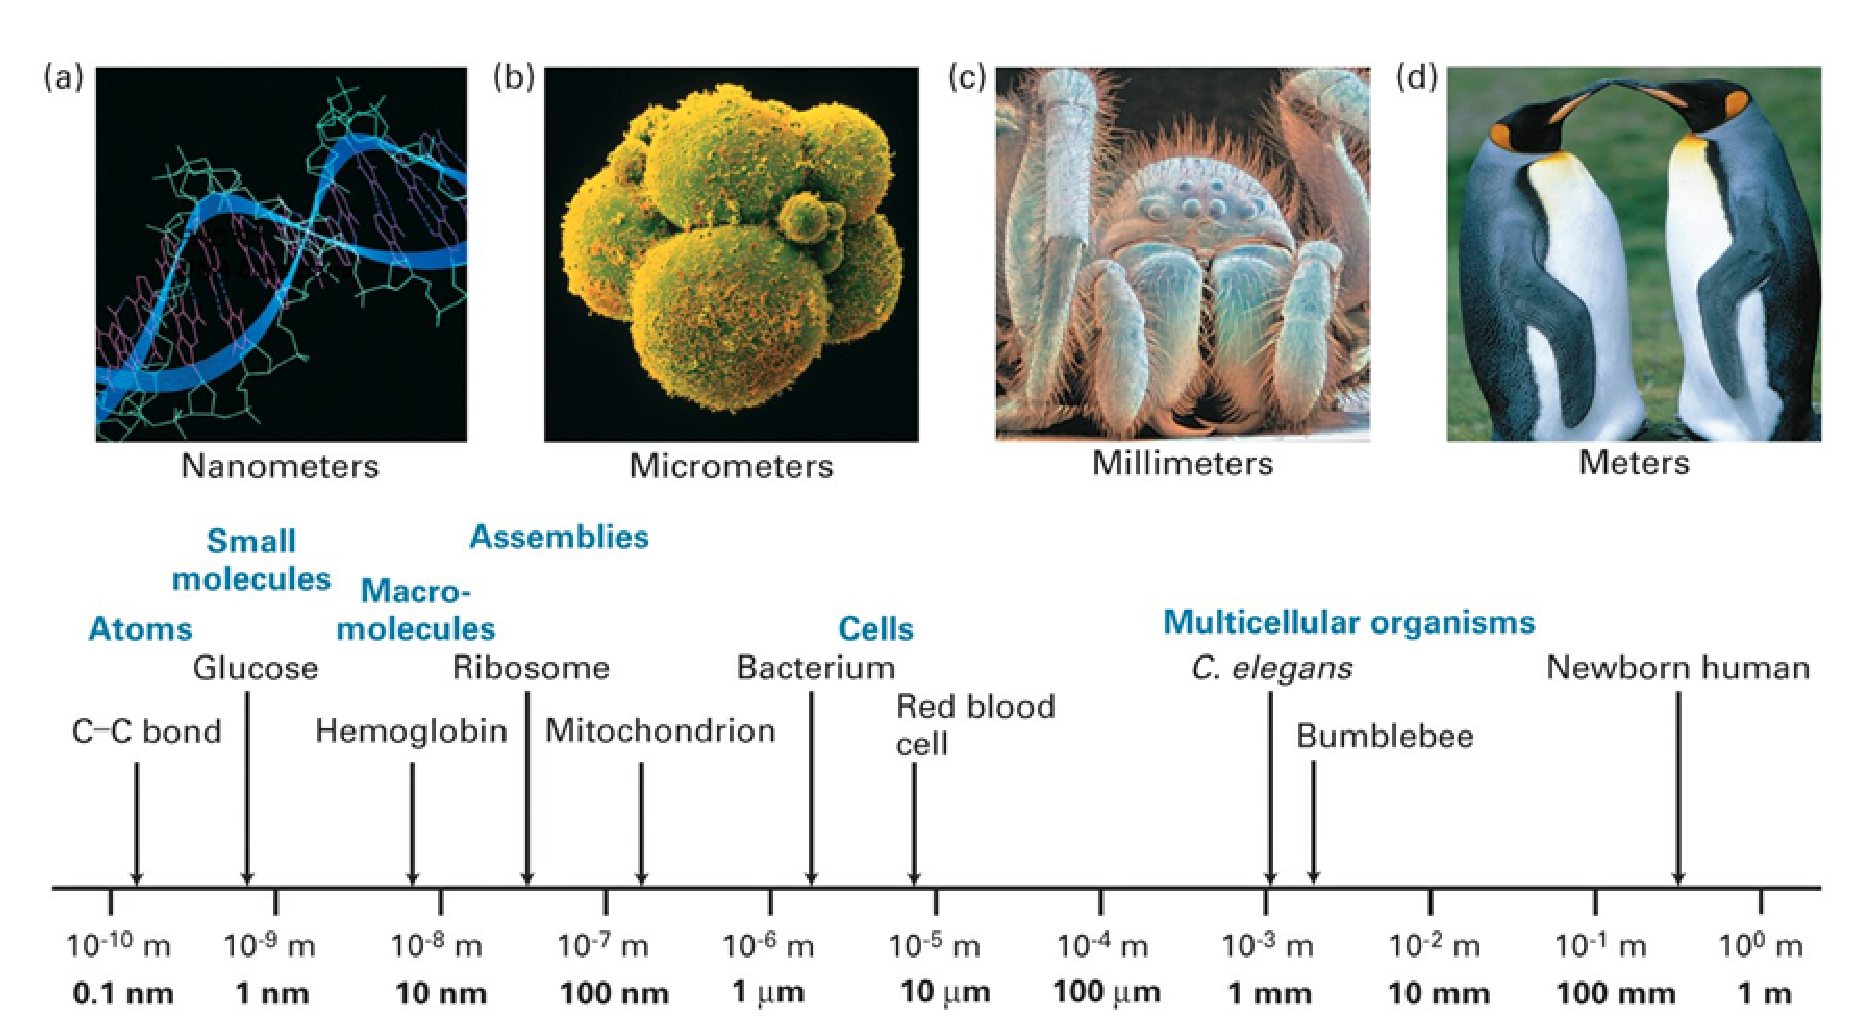
\includegraphics[height=6cm,
    angle=0]{./images/smallness.eps}}
\caption{Multi-scale of lifes}
\label{fig:smallness}
\end{figure}

\begin{enumerate}
  \item 1869: Miescher first isolated DNA molecules from white blood cell from
  pus-soaked bandages obtained from a nearby hospital.
  
  \item 1944: Avery provides evidence that DNA, rather than protein, carries the
  genetic information (using bacterial transformation)
  
  \item 1953: Watson and Crick discovered the double-helix structure of DNA
  molecules (based on X-ray results generated by Franklin and Wilkins)
  
  \item 1955: Kornberg discovered DNA polymerase - an enzyme now used to produce
  labeled DNA probes.
  
  \item 1961: Marmur and Doty discovered {\it DNA renaturation} - establishing
  the specificity and feasibility of nucleic acid hydridization reactions.
  
  \item 1962: Arber discovered the evidence for the existence of {\it  DNA
  restriction nuclease} which can cut DNA double helix at specific sites defined
  by the local nucleotide sequence - later Nathans and H.
  Smith can purified (purified from bacteria) and use in DNA sequence
  characterization (Sect.\ref{sec:DNA-restriction-nucleases}).
  
Different species of bacteria make different restriction nucleases, which
protect them from viruses by degrading incoming viral DNA.
\footnote{\url{https://www.ncbi.nlm.nih.gov/books/NBK26837/}}

  
  \item 1966: Nirenberg, Ochoa, and Khorana elucidatd {\it genetic code}. 
  
  \item 1967: Gellert discovered {\it DNA ligase} - the enzyme that join DNA
  fragment together.
  
  \item 1972-1973:  Boyer, Cohen, Berg, and their colleagues at Stanford
  University and the University of California at San Francisco discovered {\it
  DNA cloning techniques}
  
  \item 1973: Southern discovered technique - which named after him - to detect
  the presence of a specific DNA sequence - Sect.\ref{sec:Southern-blotting}
  
  \item 1975-1977: Sanger and Barrell and Maxam and Gilbert discovered technique
  to quickly sequence DNA, i.e. rapid DNA-sequencing methods.
  
  The next generation is not available until 1991.
  
  \item 1981-1982: Palmiter and Brinster produced {\bf transgenic mices};
  Spradling and Rubin produce transgenic fruit flies.
  
  \item 1982: GeneBank was created, at  Los Alamos National Laboratory, to store 
  publicly available sequenced genetic DNA sequences.
  
  \item 1983: Murray and Szostak described YAC - Sect.\ref{sec:YAC}
  
  \item 1985: Mullis and co-workers invented {\bf PCR} - Sect.\ref{sec:PCR} 
  for fast DNA cloning
  
  \item 1987: Capecchi and Smithies introduced technique to perform {\bf
  targeted gene replacement in mouse embryonic stem cells.}
  
  \item 1989: Fields and Song developed {\bf yeast two-hybrid system} - study
  protein-protein interactions - Sect.\ref{sec:protein-protein-interaction}
  
  
  \item 1989: Olson and colleagues describe sequence-tagged sites, unique
  stretches of DNA that are used to make physical maps of human chromosomes.
  
  \item 1990: Lipman and colleagues release {\bf BLAST} - algorithm to  search
  for homology between DNA and protein sequences.
  
  \item 1990: Simon and colleagues studied how to efficiently use BAC
  (Sect.\ref{sec:BAC}) to carry large pieces of cloned human DNA for sequencing.
  
  \item 1991: Hood and Hunkapillar introduced new automated DNA sequencing.
  
  \item 1995: Venter and colleagues sequenced the {\it first complete genome} -
  and from bacterium Haemophilus influenzae.
  
  \item 1996: Goffeau and an international consortium of researchers announced
  the {\it first complete genome of a eukaryote} - from yeast Saccharomyces
  cerevisiae.
  
  The one for human is in 2001.
  
  \item 1996-1997: Lockhart and colleagues and Brown and DeRisi produced {\bf
  DNA microarray technique} - allow the simultaneous monitoring of thousands of
  genes.
  
  \item 1998: Sulston and Waterston and colleagues produced {\it the first
  complete sequence of a multicellular organism} - from nematode worm
  Caenorhabditis elegans.
  
  \item 2001: Consortia of researchers announced the {\it first draft of
  sequenced human genome}
\end{enumerate}

\subsection{DNA: deoxyribonucleic acid}
\label{sec:dna}
\label{sec:amino-acid}


DNA  -  deoxyribonucleic acid  -  is the material for genes, Fig.\ref{fig:DNA}.

\begin{itemize}

 \item DNA is the polymer formed by the sequence of monomers called {\bf
  nucleotides} - Sect.\ref{sec:nucleotide}. There are 4 different types of
  nucleotides (Sect.\ref{sec:nucleotide}) that make up the DNA: A, T, G, C.

A DNA exists in the form of double strands held together by hydrogen bond (a
non-covalent force). 

A nucleotide has the structure {\bf base-sugar-phosphate}. 
\begin{itemize}
  \item sugar (ribofuranoside group) - Sect.\ref{sec:ribofuranose}
  \item phosphate (phospho-diesters) - Sect.\ref{sec:phosphate-group}
\end{itemize}
A base of an amino acid in protein is encoded by a triplet of 3 adjacent
nucleotide in the DNA.

  \item  A gene is a segment of the DNA at which it carries information
  (chemical message) which holds information that signals the cell how to
  assemble the amino acids in the correct order to produce/make the protein
  (Sect.\ref{sec:protein-overview}) for which that gene is "responsible".

A triplet of 3 adjacent nucleotides (bases) on a DNA strand specifics (i.e.
encode) each amino acid in a protein. Hence, to code for large number of
proteins, the length of the DNA has to be very long.  

Genes are part of the chromosomal DNA molecule. Each gene is distinct from the
next, separated by spacer sequences  -  which has no known function.

  \item (As such information is inherited from both parents) the
  information is called {\it hereditary information} or genetic information.

 \end{itemize}

\begin{figure}[hbt]
  \centerline{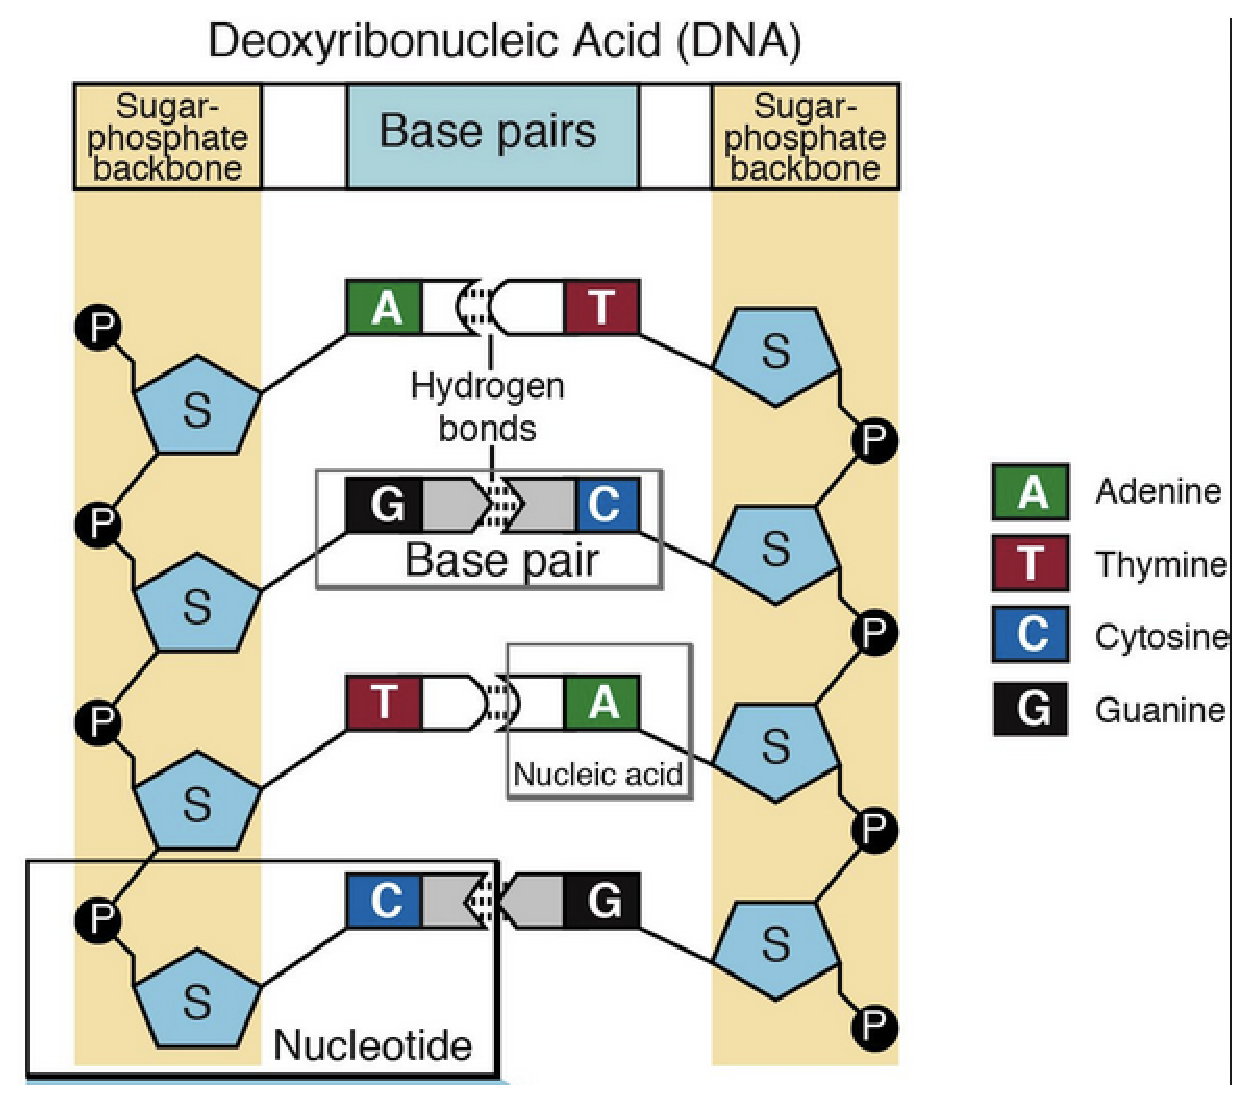
\includegraphics[height=5cm,
    angle=0]{./images/DNA.eps}}
\caption{A (double-straned) DNA with two sugar-phosphate backbone}
\label{fig:DNA}
\end{figure}


\subsection{Nucleotide (nucleobase)}
\label{sec:nucleotide}
%\label{sec:nucleotide}

A nucleobase
\begin{enumerate}
  \item {\bf A}denosine	
  \item {\bf T}hreonine
  \item {\bf G}uanine	
  \item {\bf C}ytosine ({\bf U}ranine)
\end{enumerate}

A {\bf nucleotide}, Fig.\ref{sec:nucleotide} is a monomer units forming DNA and
RNA. DNA has 4 types of nucleotides: A, T, G and C; while RNA has 4 types: A, U,
G, and C.

A nucleotide is composed of (in the direction of 5' to 3')
\begin{itemize}
  \item 5'-end (i.e. 5'-position of the carbon atom in the sugar ring):
  phosphate group (one or many)

  \item 5-carbon sugar ring:

  \item 3'-end:  nitrogeneous base (e.g.  adenine, guanine, thymine, cytosine)
\end{itemize}
A nucleotide is also called {\bf nucleobase} due to its role in bonding nucleic
acids (DNA and RNA), Fig.\ref{fig:DNA} - Sect.\ref{sec:dna}.

\begin{figure}[hbt]
  \centerline{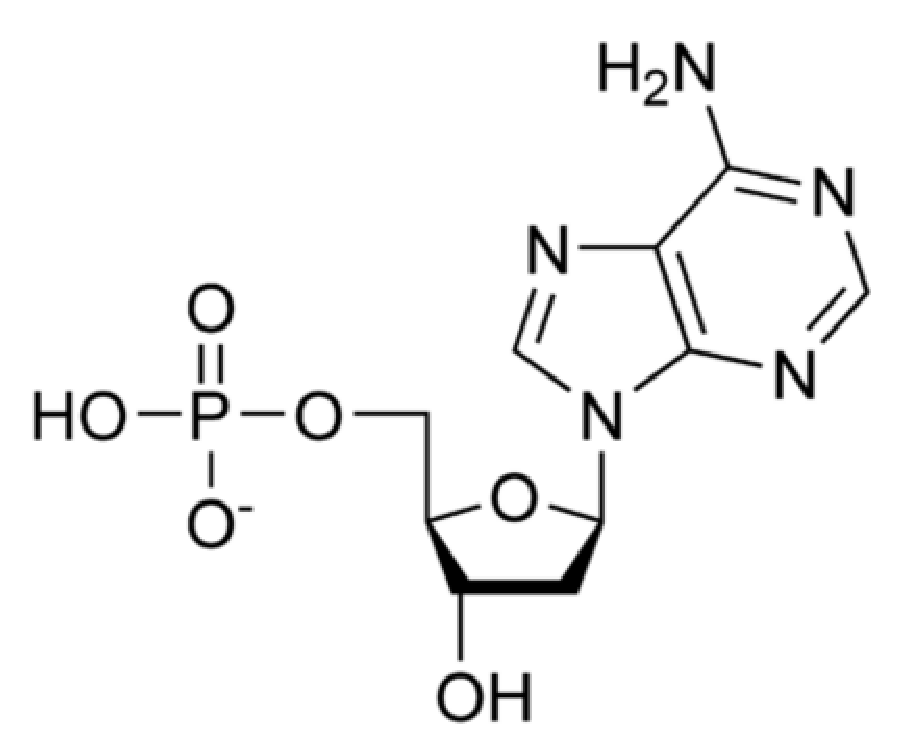
\includegraphics[height=5cm,
    angle=0]{./images/nucleotide.eps}}
\caption{A nucleotide is a building block of nucleic acids. It is a monomer
composed of (1) a nitrogenous base (whose purpose is to bond nucleic acids
together), (2) a 5-carbon sugar; and (3) a phosphate group }
\label{fig:nucleotide}
\end{figure}


\subsection{-- Adenosine (A)}
\label{sec:adenosine}



\subsection{Junk DNA: dogma of life}
\label{sec:junk-dna}


The {\bf Central Dogma} about genetic inheritance has been widely
accepted for decades. 
\begin{verbatim}
DNA --> RNA --> mRNA --> genes ---> protein 
\end{verbatim}

Now, very recently it has become evident that our concept of genetic inheritance
is not the full story. First, biological complexity is not proportional to gene
numbers. The rice plant has more genes than does a human. Another oddity is
that, in a human, the DNA sequences that actually code for protein sequences
amount to only 1.5\% of the total. What happens to the rest?

A large amount of the DNA have no (or unknown) informational
content. So, this major part in a DNA sequence is called
{\bf junk DNA}. Until recently, there is now evidence that junk DNA
contains large number of {\it non-coding microgenes}. They code for
tiny micro RNAs which are not for protein-coding purposes. What are
they for?

It is too early to be known fully but tiny micro RNAs appear to be
responsible for some of the inherited characteristics of
organisms. Elimination of microgenes has been shown to cause dramatic
changes in the structure of a plant. This is a hot research area of
molecular biology.


\section{RNA: mRNA (microRNA), rRNA, tRNA}
\label{sec:RNA}

Although DNA stores the information which cells utilize for protein synthesis.
This is a multi-step process, and the first one is generating RNA. In other
words, RNA carries out the instructions encoded in DNA. Importantly, the
process needs the help of a special protein - called {\it RNA polymerase}
(Sect.\ref{sec:RNA-polymerase}).

\begin{verbatim}

DNA (double strand) ---[transcription]--->        RNA
RNA (single strand) ---[copy         ]--->        RNA
\end{verbatim}

A RNA is a linear, single-stranded polymer, composed of ribose nucleotides, that
is synthesized by transcription of DNA or by copying of RNA. This process is
called {\bf transcription}
\begin{equation}
\ce{ \text{a segment of DNA (double-strand)} ->[\text{enzyme RNA polymerase}]
RNA}
\end{equation} 

\begin{equation}
\ce{RNA ->[\text{copy}] RNA}
\end{equation}

Both RNA and DNA are nucleic acids. In the first method, the RNA
polymerase bind and open the double strand from the 5' end (i.e. DNA
upstream) at a specialized sequence called {\bf promoter} (which is about 3
elements in bacteria, but upto 7 elements in eukaryote). \textcolor{red}{This
promoter is not so far from the site or location of transcription initiation}.

\begin{itemize}
  \item TATA box (TATTAA sequence): in eukaryote is about 25-35 base pairs away
  from the transcription initiation site.
  
  \item TATAAT sequence (called Pribnow box) in prokaryote is about 10 base
  pairs away from the transcription initiation site
   
   NOTE: Not all Pribnow box has this exact sequence TATAAT. This is just the
   most common sequence. 	
   
   \item TTGCCA sequence which is about 35 base pairs upstream from the
   transcription initiation site.
   
\end{itemize}
\url{http://www.nature.com/scitable/topicpage/dna-transcription-426}

Many eukaryotic genes also possess an enhancer sequence, which is at a
considerable distance from the genes they effect. NOTE: Some genes have an A-T
rich region of 40-60 nucleotides upstream from the transcription initiation site
that enhance the rate of transcription. The enhancer sequence binds to activator
protein and alter the 3D structure of the DNA to help the DNA 'attract' the RNA
pol II easier. REMEMBER: The eukaryotic DNA are not straight, but is tightly
packed as chromatin, and thus it needs some specialized proteins to make the
template strand accessible.

\subsection{RNA polymerase}
\label{sec:RNA-polymerase}

There are 3 different kinds of RNA polymerase in eukaryotic cells (but only 1
in bacteria) which then create three types of cellular RNA - mRNA, rRNA, and
tRNA - play different roles in protein synthesis.

\begin{enumerate}
  \item RNA pol I: transcribe genes that encode ribosomal RNA (rRNA).
  
  rRNA then associate a set of proteins to form ribosomes.
  
  A ribosome is a large complex comprising several different rRNA molecules and
  more than 50 proteins, organized into a large subunit and small subunit; the
  site of protein synthesis.
  
  
  \item RNA pol II: transcribe genes that encode messenger RNA (mRNA) - which
  serves as the templates for production of protein. The protein synthesis occur
  at ribosome. The genes transcribed by the RNA pol II are also called pol II
  genes.
  
  The information is encoded in the form of a series of 3-base code 'words',
  each 3-base (called {\bf codon}) encodes an amino acid in a protein. Which
  3-base map to which amino acid is decided by the tRNA
  
  There are 4 different types of base: 
  \begin{itemize}
    \item DNA: has A, C, G, T : adenine, cytidine, guanine, and thymine
    \item RNA: has A, C, G, U : adenine, cytidine, guanine, and uracil
  \end{itemize}
  So, 1-base system encode only 4 amino acids, 2-base system encode 16 amino
  acids. With 20 amino acids, it requires a 3-base system which can encode 64
  code words. But there are only 20 amino acids, i.e. 20 code words. So, among
  64 code words
  \begin{itemize}
    \item 3 code words are used to encode the stop codon, i.e. telling to stop
    the synthesis
    
    \item 61 code words to encode for 20 amino acids. So, most amino acids are
    encoded by more than one codons.
  \end{itemize}
  
  \item RNA pol III: transcribe genes that encode transfer RNA (tRNA).
  tRNA is the key to deciphering the code words in mRNA.
  
  Each type of amino acid has its own type of tRNA, which binds it and carries
  it to the growing end of a polypeptide chain if the next code word on mRNA
  calls for it.
  
\end{enumerate}
\url{http://www.ncbi.nlm.nih.gov/books/NBK21603/}

\subsection{microRNA (miRNA)}
\label{sec:microRNA}
\label{sec:mRNA}

The mRNA is processed in the nucleus before transport to the cytoplasm.

MicroRNAs (miRNAs) are small (17-24 nucleotides) non-protein coding genes
present in virtually all animals and  plants;  and tend to be transcribed from
several different loci in the genome.

Though not encoding for protein, MicroRNAs  mediate post-transcriptional gene
silencing by binding to the 3'-untranslated region (UTR) or open reading frame
(ORF) region of target mRNA. The discovery of microRNAs as well as other RNAs
that do not encode for proteins, indicates that there is much more to the genome
than protein coding genes. Indeed, microRNAs represent ~4\% of the genes in the
human genome.

This discovery suggests that the genome is far from being deciphered, and most
importantly that miRNAs are likely to represent just the "tip of the iceberg"
with many other small non-coding RNAs to be discovered.

miRNA are found in exosome (Sect.\ref{sec:miRNA-in-exosome}).
Given the transportability of vesicles (Sect.\ref{sec:exosome}), the role of
miRNAs in exosomes is gaining increasing attention.

\subsection{-- mRNA level to protein expression}
\label{sec:mRNA-level-2-protein-expression}

{\bf How is mRNA expression predictive for protein expression?} 
A key assumption in studying mRNA expression is that it is informative in the
prediction of protein expression. However, only limited studies have explored
the mRNA-protein expression correlation in yeast or human tissues and the
results have been relatively inconsistent.   

\begin{enumerate}
  \item  the first multilevel expression correlation study in normal human
  cells, human circulating monocytes (CMCs) (Guo et al., 2008).
  
  CMCs are an important cell type in the human immune system.
  The protein expression level is studied using 2-DE gels for quantification and
  identification. Here, 105 protein spots were detected and the intensity of the
  gray scale represent the expression level.
  The result showed that mRNA expression might be sometimes useful, but
  certainly far from perfect, in predicting protein expression levels.
  
  \item Kendrich et al. (2014) 
  
  \item 
\end{enumerate}

% Acta Biochim Biophys Sin (Shanghai). 2008 May;40(5):426-36.
% Guo Y1, Xiao P, Lei S, Deng F, Xiao GG, Liu Y, Chen X, Li L, Wu S, Chen Y, Jiang H, Tan L, Xie J, Zhu X, Liang S, Deng H.


\subsection{tRNA}

\subsection{rRNA}

\subsection{piRNA (piwi-interacting RNA)}
\label{sec:piRNA}


\subsection{siRNA}
\label{sec:siRNA}


\subsection{intron-derived miRNA (miRtrons)}
\label{sec:miRtrons}



\section{Chromosome}
\label{sec:chromosome}

A chromosome = thread-like structure of nucleic acids (i.e. DNA sequences) and
protein {\it found in the nucleus of most living cells}, carrying genetic
information in the form of genes - Sect.\ref{sec:gene-history}.
The protein - histone (Sect.\ref{sec:histone})


\subsection{chromosome 4}
\label{sec:chromosome-4}

Chromosome 4 spans more than 186 million base pairs (the building material of
DNA) and represents between 6 and 6.5 percent of the total DNA in cells.

Chromosome 4 likely contains 1,000 to 1,100 genes that provide instructions for
making proteins. Changes in chromosome 4 have been identified in
\begin{enumerate}
  \item several types of human cancer

genetic changes are somatic, which means they are acquired during a person's
lifetime and are present only in certain cells

A specific translocation involving chromosome 4 and chromosome 14 is commonly
found in multiple myeloma, which is a cancer that starts in cells of the bone
marrow, e.g. abnormally fuses the WHSC1 gene on chromosome 4 with part of
another gene on chromosome 14, leading to overactive WHSC1, which appears to
promote the uncontrolled growth and division of cancer cells.
  
  \item Facioscapulohumeral muscular dystrophy:  

  \item WHS (Wolf-Hirschhorn syndrome):
  a contiguous gene deletion syndrome associated with a hemizygous deletion of
  chromosome 4p16.3.
  
  \url{http://www.omim.org/entry/194190}
  
  
  \item \url{https://ghr.nlm.nih.gov/chromosome/4#conditions}
\end{enumerate}


\section{Biomolecule: organic compounds}
\label{sec:living-organisms}
\label{sec:biomolecule}

NOTE: Please check out the movie "{\it The inner life of a cell}" created in
NewTek Lightwave 3D and Adobe after
Effect\footnote{\url{http://www.studiodaily.com/main/searchlist/6850.html}}

\begin{framed}
  Living organisms are complicated (with multi-scale structures) but highly
  organized (Sect.\ref{sec:incredibility-life}).
\end{framed}

A typical organism is composed of many {\bf cells} (typically of many types)  -
viruses excluded. In turn, these cells possess subcellular structures (known as
{\bf organelles}). Even though small, organelles subsequently are complex
assemblies of very large {\bf polymeric molecules} (known as macromolecules).
A {\bf macromolecule} has a complex three-dimensional structure (the
conformation) which is a consequence of interactions/bonding between the {\bf
monomeric units} (small molecules such as sugars, amino acids, and lipids)
according to their individual chemical properties.

\begin{framed}
  Sugars (Sec.\ref{sec:sugar}), Amino Acids (Sect.\ref{chap:amino-acids}),
  Lipids (Sect.\ref{sec:lipids}) are all basic molecules for creating living
  cells.
\end{framed}

\subsection{Aldehydes vs. Ketones}
\label{sec:aldehydes}
\label{sec:ketones}

A {\bf aldehyde} is an organic compound with the carbonyl structure (i.e.
central carbon bonded to a hydrogen and R-group) $\ce{R-CHO}$; and 
the carbonyl is placed at the end of the carbon skeleton.

A {\bf ketone} also has the carbonyl structure like aldehyde, yet the 
carbonyl is placed in  between two carbon atoms of the backbone.



Aldehydes and ketones are widespread in nature and are often combined with other
functional groups. Aldehydes and ketones are known for their sweet and sometimes
pungent odors.

\url{http://chem.libretexts.org/?title=Core/Organic_Chemistry/Aldehydes_and_Ketones/Properties_of_Aldehydes_&_Ketones/Natural_Occurrence_of_Aldehydes_and_Ketones}
\subsection{Important role of H, N, C and O}
\label{sec:important-role-h}

{\bf CHONPS}: mnemonic acronym for the most common elements in living
organisms: carbon, hydrogen, oxygen, and nitrogen, phosphorus, sulfur.

\begin{figure}[hbt]
  \centerline{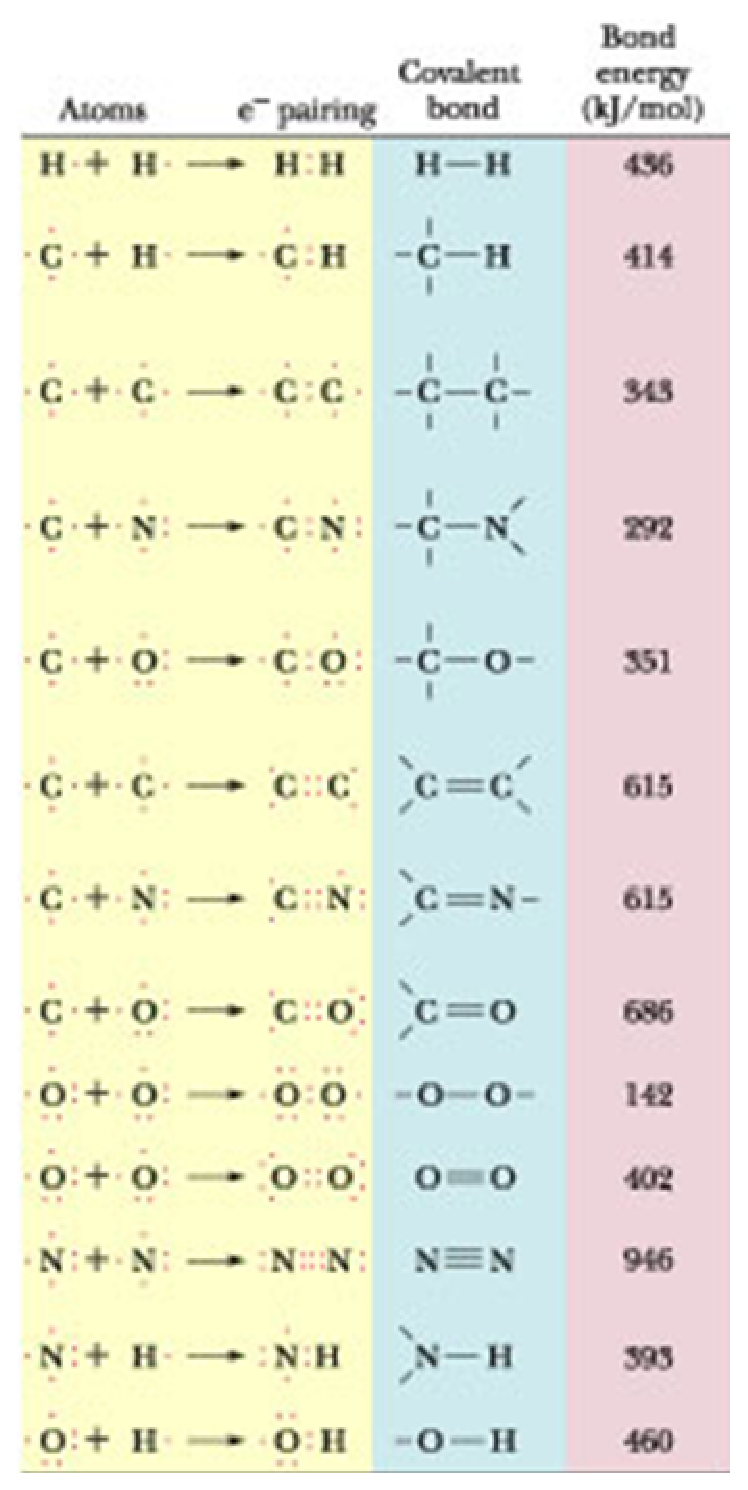
\includegraphics[height=10cm,
    angle=0]{./images/bonding_C.H.O.N.eps}}
  \caption{Bonding C, H, O, N}
  \label{fig:bonding_chon}
\end{figure}


\begin{framed}
  In those basic molecules described above, H, N, C and O are
  important to the chemistry of life; especially C which forms the
  backbone of all biomolecules. 
  
  As C can bond readily to other C atoms; they can build an arbitrarily long
  complex molecules and polymers. 
  
  In the periodic table, a molecule with similar properties with C is Si
  (silicon) - with 4 valence bonds and can bonds to itself in the form of
  crystal lattices (rather than long chains like C). However, 
  Silicon compounds do not readily recombine into different permutations in a
  manner that would plausibly support life-like processes.
\end{framed}

Beside their very abundance in nature, H, N, C and O can form covalent
bonds (strong) by electron-pair sharing. Furthermore, they are
{\it among the lightest elements of the periodic table} capable of
forming such bonds. 

Biomolecules are macromolecules, normally in the form of polymers,
i.e. long chain of monomers (amino acid, nucleotide...). In such
biomolecules, carbons (C) are the backbone. The reason is that C atoms can
form 4 covalent bonds (maximum) with other atoms, together with its
ability to form C-C bonds, enables the formation of a wide variety of
molecules of different shapes, size and properties.


\subsection{History }
\label{sec:history-}

\subsection{-- urea: first synthesized organic compound}

In 1828: urea  is the first organic compount  to be synthesized artificially (from inorganic materials)
\begin{itemize}
\item	urea is the waste product (found and retracted from urine)
 \item	urea is highly soluble (it can create 6 hydrogen bonds with water)
 \item	too high concentration of urea in the blood can cause damage to organs in the body

\end{itemize}

\subsection{-- enzyme (-ase) is protein?}
\label{sec:enzyme-history}

In 19th century, when studying the fermentation of sugar to alcohol by
yeast, Louis Pasteur recognized that this process occurs under a vital
force contained within the yeast cells called "ferments". In 1878,
Wilhelm Kuhne coined the term enzyme (come from Greek "in leaven") to
describe such process.

In 1897, Eduard Buchner produced cell-free yeast extract and used this
"press juice" to show that sugar was fermented even when there is no
living yeast cells. It means that the fermentation process does not
occur inside the yeast cells. He call such yeast extract zymase.
\begin{itemize}
 \item Later on, various enzymes are named according to the reaction
   they carry out. Typically the suffix \verb!-ase! is added to the
   name of the substrate (e.g., lactase is the enzyme that cleaves
   lactose) or the type of reaction (e.g., DNA polymerase forms DNA
   polymers).

  \item Buchner hypothesized that yeast cells secrete proteins into
    their environment in order to ferment sugars.
\end{itemize}

At this point, we all know that enzyme could function outside a living
cells. However, there were arguments that proteins are not enzymes,
they are merely carriers for true enzymes and that proteins per se are
incapble of catalysis. In 1926, Sumner showed that enzyme urease was a
pure protein. In 1937, he showed the same result with enzyme
catalase. And the affirmative conclusion was finally proved by
Northrop \& Stanley: enzymes are proteins.

\subsection{-- lysozyme: first resolved structure enzyme}
\label{sec:lysozyme-history}

At that days, proteins has very small structure that cannot be seen by
microscope. Hence, their structures were unknown. However, the
discovery that enzymes can be crystallized eventually allowed their
structures to be identified by the X-ray crystallography technique. In
1965, the first enzyme's structure to be solved was lysozyme (an
enzyme found in tears, egg whites that digests the coating of some
bacteria * kill the bacteria).

\subsection{-- metabolism process}

Metabolism is the term derived from Greek metabolimos for "change" or
"overthrow". The first metabolic cycle discovered was the urea cycle (discovered
by Krebs). The next very important metabolic cycle was the cytric acid cycle
(Krebs cycle).

\subsection{-- gene}
\label{sec:gene-history}

Another historic event is the discovery of {\bf genes} and its role in the
transfer genetical information. {\it A gene is a stretch of DNA or RNA that
determines a certain trait.} 

There is always two copies of a gene - one on the chromosome from the mother,
and one from the father. The exception is genes on the X and Y chromosomes.

Genes mutate and can take two or more alternative
forms
\begin{enumerate}
  \item allele - Sect.\ref{sec:allele}: variants in gene (i.e. DNA sequencing)
  that encode for the same trait.

Each organism has two alleles for every gene, one on each chromosome.


  \item
\end{enumerate}

In 1958, Beadle \& Tatum received the Nobel prize for work in fungi showing that
one gene produces one enzyme (or protein). Even though all cells hold the
same genetic information (stored in chromosomes - Sect.\ref{sec:chromosome}),
depending on the cell type, certain genes are expressed while some are
silent. The question is on which cell type a gene is expressed and at what
level (Sect.\ref{sec:gene-transription-process}).

Since then, the biochemistry has advanced with the development of new techniques
such as chromatography, X-ray diffraction, NMR spectroscopy, radioisotopic
labelling, electron microscopy and molecular dynamics simulations.  Today, there
are 3 branches of biochemistry (as established by Michael Sugar)

\begin{itemize}
  \item Plant biochemistry
  \item General biochemistry
  \item Human/medical/medicinal biochemistry (focus on the biochemistry of human and medical illness)
\end{itemize}

\subsection{-- allele}
\label{sec:allele}

Humans, have paired homologous chromosomes in their somatic cells, and these
contain two copies of each gene. An organism in which the two copies of the gene
are identical - that is, have the same allele - is called homozygous for that gene. 

For heterozygous, {\bf condominance} is the situation in which two different
alleles for a trait are expressed unblended in the phenotype of heterozygous
individuals.  Neither allele is dominant or recessive, so that both appear in
the phenotype or influence it.  Type AB blood is an example.  Such traits are
said to be codominant.

A {\bf dominant allele} is an allele that masks the presence of a recessive
allele in the phenotype. Dominant alleles for a trait are usually expressed if
an individual is homozygous dominant or heterozygous.

{\bf Incomplete penetrance} is the situation in which an allele is expressed
only if certain factors are present in the environment.



An {\bf allele} is a specific variation (or mutation) of a gene.
Example: each person has 23 pairs of chromosomes.
Suppose we choose a particular chromosome from two different people and examine
the DNA from the same spot on both chromosomes. We will find that the pattern of
the bases (A's, C's, T's, and G's) is similar, but it is often not exactly the
same, even if the region is a protein-coding gene. So, {\bf there can be
different variant of a gene that can encode for a given product, e.g. eye
color}. Different alleles of a single gene code for the same trait, but they may
manifest themselves in different ways. The gene for eye color contains the
instructions governing eye pigment, for example, but the specific color is
determined by the particular alleles one has. 

{\bf Example}: the gene for eye color has several variations (alleles) such as
an allele for blue eye color or an allele for brown eyes.

{\bf Example}: The way in which the Huntington gene varies among individuals is
by the number of repeated C-A-G codons it contains. t is important to understand that
everyone has the Huntington gene, but individuals with Huntington's disease have
a many-CAG version of the gene, one that does not function normally.
\url{http://web.stanford.edu/group/hopes/cgi-bin/hopes_test/the-inheritance-of-huntingtons-disease-text-and-audio/#what-are-alleles-how-many-alleles-can-there-be-for-a-gene-and-how-many-copies-does-each-individual-have}

Each organism has two alleles for every gene, one on each chromosome.
{\bf The body/cell will uses one allele to express the protein.} (the question
is which one, see below). If the two alleles are the same (e.g., both coding for
blue eyes), they are called {\bf homozygotes}. If they are different (e.g., one for blue eyes and one
for brown eyes), they are {\bf heterozygotes}.  In the case of heterozygotes,
the individual may "express" either one or a combination of the two traits.
\begin{enumerate}
  \item A dominant allele is one that will always be expressed if present. 
  
  For example, the allele for Huntington's disease is dominant, so if an
  individual inherits an allele for Huntington's from only one of the parents,
  they will have the disease. 
  
  \item a recessive allele is one that will only be expressed if it is found on
  both genes.
\end{enumerate}
A person actually has two copies of every gene, one allele on each of two
homologous chromosomes. 
\begin{verbatim}
Allels present               Allele expressed
Dominant/Dominant -->         Dominant
Dominant/Recessive-->         Dominant
Recessive/Recessive-->        Recessive
\end{verbatim}

Since each chromosome in the pair comes from a different parent, organisms
inherit one allele from each parent for each gene. 

\subsection{-- protein synthesis rate}

Protein biosynthesis is by far the largest consumer of energy during cellular
proliferation; translation by ribosomes is estimated to account for ~50\% of the
energy consumption of a rapidly growing bacterial cell, and ~30\% of that for a
differentiating mammalian cell (Buttgereit and Brand, 1995; Russell and Cook,
1995).  Eukaryotic cells have mechanisms to ensure that the products of
so-called {\bf housekeeping genes}, which are needed in great abundance, are
available to the cell.
\begin{itemize}
  \item   One method is to attract and keep the RNA polymerases (which
  transcribe the gene into messenger RNA (mRNA), which is the template for
  translation into a protein - the actual gene product) bound to the gene
  sequence through a variety of DNA "promoter" and "enhancer" sequences, which
  other proteins called transcription factors bind to and recruit the polymerase
  to the gene. These polymerases are kept active for as long as the cell needs
  the gene's protein product, churning out copy after copy of mRNA      
  
  \item There are many other mechanisms as well, ranging from how the core
  histone proteins that give chromosomes their shape bind near the gene, to the
  manner in which the translation machinery (ribosomes) bind to the mRNA and
  produce multiple protein molecules per mRNA copy.   
\end{itemize}
\url{https://www.ncbi.nlm.nih.gov/pmc/articles/PMC4006352/}



\subsection{Numbers in Greeks}
\label{sec:numbers-greeks}

The names of organic compounds are often given by the length of the
carbon chain. 
\begin{itemize}
\item Di-   = 2
\item Tri-  = 3
\item Penta- = 5
\item Hexa- = 6
\item Octa- = 8
\item Deca- = 10
\item Octadeca- = 18
\item 
\end{itemize}

\section{Phosphate group}
\label{sec:phosphate-group}


A phospshate group ($\ce{-PO4^-}$) has many important roles.
Along with sugars (Sect.\ref{sec:sugar}) and bases (Sect.\ref{sec:bases}), i.e.
the sugar-phosphate backbone, it makes up nucleic acids, like DNA and RNA
(Sect.\ref{sec:dna}). As part of energy carriers, like ATP, it provides energy
for moving our muscles.

In addition to its role in the backbone of DNA, phosphate groups play a
biochemical role in ribosome-substrate interactions and the regulation of
cellular processes. Phosphate groups also play a major part in the bending of
the DNA backbone, due to the repulsion of the negative charges. 


\section{Isomers: constitutional isomers + steroisomers}
\label{sec:isomer}

{\bf Isomers} are molecules with the same chemical formula, but differ
chemical structure, i.e. individual atoms are arranged differently in space.



The two main forms
\begin{itemize}

  \item {\bf Stereoisomer} = isomers, with the same sequence of bonded atoms,
  but differs in 3D  orientations, i.e. atoms have different arrangement of
  atoms (Sect.\ref{sec:stereoisomers}).
  
  \item {\bf Structural isomers} (constitutional isomers) = isomers, but with
  different order of the bond connections.
\end{itemize}
We will focus on steroisomers, e.g. cis-trans isomers (Sect.\ref{sec:cis-}).

\url{http://chemwiki.ucdavis.edu/Inorganic_Chemistry/Coordination_Chemistry/Isomers/Stereoisomers}

\subsection{Stereoisomers}
\label{sec:stereoisomers}

Stereoisomerism is the arrangement of atoms in molecules whose connectivity
remains the same but their arrangement in space is different in each isomer. The
two main types of stereoisomerism are: {\bf DiaStereomerism} (including
'cis-trans isomerism') and {\bf Optical Isomerism} (also known as
'enantiomerism' and 'chirality' - Sect.\ref{sec:enantiomers})

Stereoisomerism can occur when a double bond is present, because the pi bond
involved prevents that bond from being "twisted" the same way as single bond.


Diastereomers are stereoisomers that are not enantiomers (mirror images) of each
other. With different shapes, diastereomers can have different physical and
chemical properties. 

\subsection{-- Diastereomer}
\label{sec:diastereomer}



\subsection{------ cis- and trans-isomers (geometric isomer)}
\label{sec:cis-}
\label{sec:trans-}


{\bf Cis-trans isomers } (obsolete term: geometric isomeris) = isomers with
restricted rotation molecules, e.g. due to double bonds. {\bf Geometric
isomerism} concerns the type of {\it isomer} where the individual atoms are in
the same order, but manage to arrange themselves different spatially.
We will focus on the cis-trans isomers in {\bf biomolecules}.

The cis/trans system should only be used when the carbon atoms involved each
have a hydrogen atoms attached. The prefix {\bf cis-} and {\bf trans}- are used
to identify which side of the double bond C=C the similar atoms are found,
Fig.\ref{fig:Cis-Trans}.
\begin{enumerate}
  \item cis- = on-this-side (two functional groups connecting to each C-atom  of
  the double-bond link are on the same side of the double bond C=C)
  
  \item trans- = across (two functional groups are on opposite side of the
  double bond C=C)
\end{enumerate}
The trans/cis system for naming isomers breaks down when there are more than two
different substituents on a double bond, and thus E/Z notation is used
(Sect.\ref{sec:E-Z-notation})

\begin{mdframed}
{\bf Biomolecules} are complex molecules with C-C or C=C connections as the
backbone and attach to the backbone are functional groups.
\begin{itemize}
  \item C-C = single-bonding of two carbon atoms
  \item C=C = double-bonding of two carbon atoms
  
  Double bonds are formed when p orbitals between two atoms overlap.
  \textcolor{red}{Double bond restrict free rotation}.
\end{itemize}
IMPORTANT: If there are two identical functional groups on one side of the
carbon link, the biomolecule cannot be an isomer, e.g. $\ce{(CH3)2C=CClCH3}$.

\end{mdframed}
%Depending on the orientation of the functional groups



\begin{figure}[htb]
    \centerline{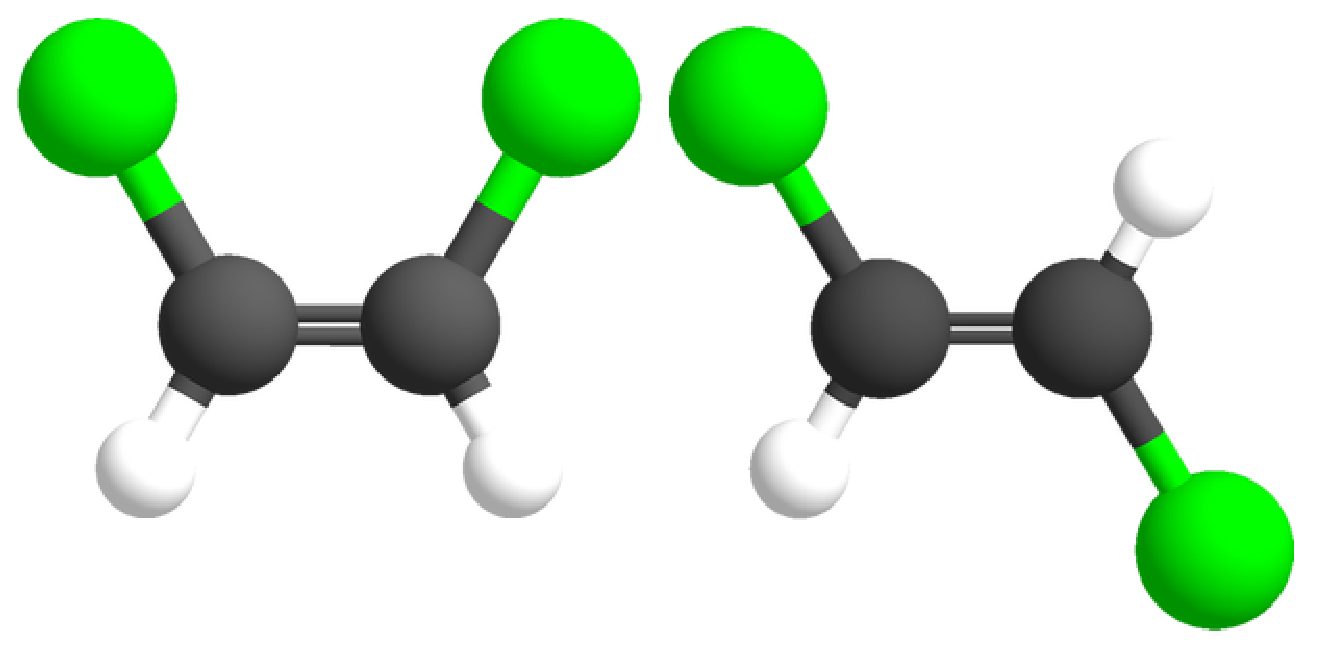
\includegraphics[height=5cm]{./images/Cis-Trans.eps}}
\caption{(Left) Cis- ; (Right) Trans-}\label{fig:Cis-Trans}
  \end{figure}

PHYSICAL PROPERTIES:
\begin{itemize}
  \item Cis- isomers tend to have {\it higher boiling points} than their trans-
  counterparts. 
  
  Trans- isomers generally have lower melting points and have lower
  densities than their cis- counterparts.
  
  \item Cis- isomers collect the charge on one side of the molecule, giving the
  molecule an overall {\it polar effect}. 
  
  Trans- isomers balance the individual dipoles and have a non-polar tendency.
\end{itemize}  
\url{http://chemistry.about.com/od/organicchemistry/tp/Geometric-Isomerism.htm}

\subsection{D- and L-form}
\label{sec:D-and-L-form}
\label{sec:L-isomer}
\label{sec:D-isomer}
\label{sec:chiral-center}


Students who take biochemistry are exposed to an old, confusing, and often
incorrect method of specifying configurations at {\bf chiral centers} as D or L.
This scheme was devised in the early years of this century by Emil Fischer, a German
organic chemist who worked extensively with carbohydrates.
\url{http://chemistry.umeche.maine.edu/CHY251/dlwrong.html}


Modern notation are R- and S-form; but it will NOT always work out that D = R
and L = S.
\begin{itemize}
  \item {\it D-=(Latin) dexter = right, L-=(Latin)laevus = left})
  \item {\it R-=(Latin) rectus = right-handed, S-=(Latin) sinister =
  (left-handed)}
\end{itemize}

\subsection{E- and Z-form}
\label{sec:E-Z-notation}

The E/Z notation is unamibiguous. Z (from the German {\it zusammen}) means
together and usually corresponds to the term cis; E (from the German
{\it entgegen}) means opposite and usually corresponds to the term trans.

RULES: for each functional group, find the 'first' one based on priority rule
\begin{enumerate}
  \item Priority rule (used to identify which part of the molecule to consider
  first)
  
  Cahn-Ingold-Prelog (CIP) priority rule: An atom with higher atomic number has
  higher priority. (e.g. I > Cl > C > H)
  
  
  \item first atom of two groups is the same, consider the second atom(s) in the
  same way as the first. (e.g. -C(CH3)3 > -CH(CH3)2 > -CH2CH3 > -CH3). If this
  does not assign priority, consider the next atoms until there is a difference.
  
  
\end{enumerate}

\subsection{-- Optical isomer (enantiomer, chiral)}
\label{sec:optical-isomer}
\label{sec:enantiomer}
\label{sec:chiral-center}

Enantiomers (or chirals) are two molecules of same molecules-arrangement; but
are nonsuperimposable mirror images.
NOTE: {\bf cheir} (Greek of chiral) = hand.
It similar to the person's left hand is the same as his right hand, except that
they are mirror images of each other.

{\it The most common cause of enantiomerism in organic molecules is the presence
of a stereocenter, carbon with four different groups bonded to it.}
This center carbon atom is known as {\bf chiral center}

{\bf Chiral centers} are tetrahedral atoms that have four different
substituents. 
\begin{itemize}
  \item  The most common type of chiral atom in organic molecules are
{\bf Carbons} because they can be SP$_3$ hybridized and can form four bonds.
  
  \item The other types of atoms that can be chiral are {\bf quaternary
  nitrogens}, {\bf tertiary nitrogens} that are at the bridgehead (junction) of
  a bicyclic ring system, hypervalent phosphorous (with more than three bonds),
  and hypervalent sulfur (with more than two bonds).  However, these other types
  of chiral atoms are very unusual.
  
  \item Molecules with a single chiral center are ALWAYS chiral. Molecules with
  more than one chiral center are {\it usually} (but not always) chiral.
\end{itemize}
\url{http://www.chem.sc.edu/faculty/shimizu/333/Chem_333/5a.ii.html}

\subsection{---- R- and S- system}
\label{sec:R,S-system}

Because enantiomers are different compounds, 
each must have a different name.

The R,S system is a way to distinguish between enantiomers without having to
draw them and point to one or the other, and use use the CIP priority rules
(Sect.\ref{sec:E-Z-notation}).

\begin{enumerate}
  \item Assign the priority to each of the atoms that are bounded to the
  sterocenter (1, highest to 4, lowest).
  
  
  
  \item  When drawing the 3D molecule structure: point the lowest priority (4)
  atom away from you.
  
  \item R configuration: clockwise from 1 to 2 to 3
  
  \item S configuration: counterclockwise from 1 to 2 to 3.
\end{enumerate}
\url{https://en.wikibooks.org/wiki/Organic_Chemistry/Chirality/R-S_notational_system#E-Z_Notation}


\section{Rings}
\label{sec:benzen}
\label{sec:aromatic-ring}

The most commonly encountered aromatic compound is benzene. The usual structural
representation for benzene is 6-carbon ring (i.e. a hexagon with 3
double-bonds and only Hydrogens connected to carbon).

Benzene was first isolated by Michael Faraday in 1825, from the whale oil used
in gaslights. Eilhardt Mitscherlich synthesized benzene in 1834, and showed it
to have a molecular formula of $\ce{C6H6}$.  
Many other compounds with similar properties to benzene were discovered in the
1800s, all having a low ratio of hydrogen to carbon. The low ratio indicates the
presence of double-bonds (C=C).
Since many of these molecules had pleasant aromas, they were called "aromatic
compounds." 
\url{https://www.angelo.edu/faculty/kboudrea/molecule_gallery/04_aromatics/00_aromatics.htm} 

Aromatic hydrocarbons are nonpolar, and are insoluble in water.  However, when
other atoms are substituted on the benzene ring, they may be very water-soluble.
 For instance, phenol, which has an -OH group attached to the benzene ring, is
very water-soluble.

A number of aromatic molecules are known by common names
\begin{itemize} 
  \item benzene with a -CH3 group attached is called "toluene"; 
  
  \item benzene with an -NH2 group attached is called "aniline"; 
  
  \item a benzene with a -CO2H group is called "benzoic acid," etc.
  
  \item  more complicated substituents, the benzene ring is named as a
  substituent, in which case it is called "phenyl."  For instance, an
  eight-carbon chain with a benzene ring on the third carbon is called
  "3-phenyloctane."
  
  
\end{itemize}


\subsection{Phenolic ring}
\label{sec:phenolic-ring}



\section{tyrosine}
\label{sec:tyrosine}

\url{http://www.russelllab.org/aas/Tyr.html}

\begin{mdframed}

Stratural analysis have provided the dominant role of {\it large} tyrosine
residues for mediating molecular contacts and of {\it small} serine/glycine
residues for providing space and flexibility. \citep{koide2009}

\end{mdframed}

Tyrosine:
\begin{itemize}
  \item aromatic $\rightarrow$ allow tyrosine to form stacking interaction with
  other aromatic side-chain, i.e. adhesion purpose
  
  \item partially hydrophobic $\rightarrow$ prefer to be buried in the protein
  hydrophobic core
  
  \item amino acid
  
  \item contains an active hydroxyl group $\rightarrow$ making it more likely to
  interact with non protein atoms (e.g. non-protein ligands)
\end{itemize}

Along with Serines and Threonines, Tyrosine is a target of phosphorylation by
protein tyrosine kinases (PTK) \citep{hubbard2000}, i.e. phosphate group
attached to the tyrosine to facilitate the signal transduction process. This
process is highly specific, i.e.
Tyrosine kinases generally do not work on Serines/Threonines and vice versa.

Phosphorylation of tyrosine residues (Sect.\ref{sec:tyrosine}) modulates
enzymatic activity and creates binding sites for the recruitment of downstream
signaling proteins.
Two classes of PTKs \citep{hubbard2000}
\begin{enumerate}
  \item transmembrane receptor PTKs (receptor tyrosine kinase - RTK, or
  tyrosine receptor kinase - TRK, {\bf Trk} is the name used in neurobiology -
  Sect.\ref{sec:Trk}):
  
  RTK has one extracellular domain for ligand binding, and one intracellular
  kinase domain. To perform its function, RTK needs to form dimer which requires
  the binding of ligand to stabilize the dimer. 
  The interaction between the cytoplasmic domain 
  of RTK stimulate the autophosphorylation of tyrosine, causing conformation
  change. Subsequent to this, the receptor's kinase domains are activated,
  initiating the phosphorylation signaling cascades.
  
   The activity is tightly regulated through several modes of autoregulation
  
  
  \item nonreceptor PTKs
\end{enumerate}


The versatility of tyrosine in forming intermolecular
contacts has also been exploited in surface engineering
to promote protein crystallization



\section{Exosome}
\label{sec:exosome}

Exosome (Pan) as inter-cellular messengers:
extracellular RNA communications (exRNA not only control the cell that hold it;
but it can control cells far apart via exosomes). Study of exosomes has
been mainly in cancer research, but still limited in cardiovascular research.

Endosomes (E) has inverted plasma membrane.

Susmita Sahoo
\begin{itemize}
  \item Sahoo - Losordo, Circ. Res, 2014
  
%    Circ Res. 2014 Jan 17;114(2):333-44. doi: 10.1161/CIRCRESAHA.114.300639.
% Exosomes and cardiac repair after myocardial infarction.
% Sahoo S1, Losordo DW.
  
  \item stemcell-derived exosomes: 

Stem cell first derived from bone marrow (Jacobson et al, 1951, Science)

Doppler et al., 2013. Cardiac regeneration: current therapies-future concepts
Stefanie A. Doppler, Marcus-Andre Deutsch, Rudiger Lange, and Markus
Kranecorresponding author
\url{https://www.researchgate.net/profile/Stefanie_Doppler}
\url{https://www.researchgate.net/profile/Marcus_Andre_Deutsch}
\url{http://www.professoren.tum.de/en/lange-ruediger/}

Due to the beating of the heart, stemcell transplant to the heart is hard, as
very few is retained.

Next: paracrine secretion from the cell which is 2 components: vesicles + 

Human CD34+ exosomes conditioned media (CM):
PB-derived CD34+ cells isolated from G-CSF mobilized individuals.
Extract two forms of sizes: 8nm and 60nm, which are then separated to get 60nm
(supposed to be exosomes). Then, they analyze morphological and biochemical
characteristics of these exosomes.

CD34+ exosome induce angiogenesis (i.e. forming new blood vessels). However,
exosomes is not uptake into the cell; but there are some proteins as receptors
on the membrane of the cell that exosomes bind to and trigger the events.

They injected the exosomes into the eschemic part of the blood vessil in
the limb, and the CD34+ exosome help retain the limb; which show the presence of
the blood flow to the limb with CD34+ exosomes presence.

CD34+ exosomes improve heart wall motion (Sham (i.e. normal): 35\%; block
everything:
5\%; then add CD34+ exosomes: 25\%).


\textcolor{red}{So, what make exosome special?}
\begin{itemize}
  \item RNA inside exosome
  \item the exosome itself
  \item the surface protein as receptor on the membrane of receiving cell
  (don't know which protein yet)
\end{itemize}
The author does not know for sure; and assume they are equally important.

Exosome RNA is enriched for miRNAs (30-60\%), measured using fluorescence unit
(FU). miRNA profiling of CD34+ shows CD34+ exo is enriched with pro-angiogenic
RNA. 

There are many miRNA: 126, 130, 30a, \ldots
They tested by knocking down miRNA-126 in exosome (but not specific as it also
affect others); and it shows a decrease in functions. \textcolor{red}{Not sure
why for now.}
So, they assume miR-126 is important, and directly induce pro-angiogenic gene
expression in mouse tissue.
\textcolor{red}{How about in human?} They don't find any difference in mouse and
human of this miRNA.

Papers: Ashraf 2010 paper; Ebrahim - Marban 2014.; Lim 2010. 
Khan, Koshere 2015.

{\bf Hypothesis}: exosomes from CDC convert inert fibroblast into beneficial
fibroblast.

CD34+ exosome is uptake quickly (within 1-4h) by cells in ischemic tissue; but
is not maintained (e.g. loss after 24h).
Mainly uptake by endothelical cells (87\%); and a smaller amount by
cardiacmyocytes (34\%). Fibroblast in cell culture is different from
that in vivo; though the author not sure why.

{\bf Hypothesis}: Na/K-ATPase surface protein control the uptake of exosomes.
It is important to know the protein that involve into regulating the uptake of
exosomes into the cells.


{\bf Question}: how about the role of heart-secreated exosomes (we have just
cover CDC34+ exosome only)? now found any physiological role so far.

Emanueli, C. 2016, PLoS One.

The author's goal is to built artificial exosomes with the necessary RNA (so we
don't need biologocaly released exosome) to treat cardiovascular diseases.


\item {\bf GOAL}: AAV-exosome: novel vector for myocardial gene delivery


\item {\bf GOAL}: epitranscriptomic regulation of cardiac ischemic remodeling
\begin{enumerate}
  \item a new layer of gene regulation: 
  
  \item the author found big difference in failing heart in m6A RNA methylation
  (high in failing heart)
  
  \item 
\end{enumerate}


\end{itemize}


Exosomes are 40-100 nm nano-sized vesicles that are released from many cell
types into the extracellular space, and are present in almost all biological
fluids. Exosomes were first discovered by Pan and Johnstone in 1983.
In 1989, Johnstone defined such functional vesicles as exosomes.
According to the way of vesicular secretion from cells, extracellular vesicles
can be grouped into two general classes
\begin{enumerate}
  \item microvesicles
  
  \item exosomes: released by exocytosis when multivesicular bodies (MVBs)
  fuse with the plasma membrane
\end{enumerate}

 In addition to the proteins, various nucleic acids have recently been
identified in the exosomal lumen, including mRNAs, microRNAs (miRNAs), and other
non-coding RNAs (ncRNAs). The exosomal RNA, i.e. mRNAs (Sect.\ref{sec:mRNA}) and
microRNAs (miRNAs - Sect.\ref{sec:microRNA}) in exosomes, can be taken up by
neighboring or distant cells and subsequently modulate recipient cells.

Exosomal miRNAs play an important role in disease progression, and can stimulate
angiogenesis and facilitate metastasis in cancers
Importantly, miRNA profiles of exosomes may differ from those of the parent cells.


Conveying information via circulating vesicles is deemed to be the third way of
intercellular communication that can deliver to cells further from the origin
cell. It is as essential as the cell-to-cell contact-dependent signaling
(e.g. electrical syanpse) and signaling via transfer of soluble molecule (e.g.
chemical synapse).


Several reports have shown that exosomes play important roles in immune
response, tumor progression, and neurodegenerative disorders. 

\subsection{exosomal miRNA}
\label{sec:miRNA-in-exosome}

There are four potential modes for sorting of miRNAs into exosomes, although the
underlying mechanisms remain largely unclear. 
\begin{enumerate}
  \item neural sphingomyelinase 2 (nSMase2)-dependent pathway
  
   overexpression of nSMase2 increased the number of exosomal miRNAs, and
  conversely inhibition of nSMase2 expression reduced the number of exosomal
  miRNAs (Kosaka et al. (2013))
  
  
  \item  sumoylated heterogeneous nuclear ribonucleoproteins (hnRNPs)-dependent
  pathway
  
  sumoylated hnRNPA2B1 could recognize the GGAG motif in the 3' portion of miRNA
  sequences and cause specific miRNAs to be packed into exosomes
  (Villarroya-Beltri et al. (2013))
  
  \item 3'-end of the miRNA sequence-dependent pathway:
  
   3' ends of uridylated endogenous miRNAs were mainly presented in exosomes
  derived from B cells or urine, whereas the 3' ends of adenylated endogenous miRNAs were mainly presented in B cells
  
  \item AGO2-related pathway or miRNA induced silencing complex
  (miRISC)-related pathway
  
   mature miRNAs can interact with assembly proteins to form a complex called
  miRISC.  The main components of miRISC include miRNA, miRNA-repressible mRNA,
  GW182, and AGO2. The AGO2 protein in humans, which prefers to bind to U or A
  at the 5' end of miRNAs, plays an important role in mediating mRNA
  
  Knockout of AGO2 could decrease the types or abundance of the
  preferentially-exported miRNAs, such as miR-451, miR-150, and miR-142-3p, in
  HEK293T-derived exosomes
  
  
\end{enumerate}


\section{Chromatin: nucleosome, histone}
\label{sec:chromatin}
\label{sec:histone}
\label{sec:nucleosome}

The eukaryotic DNA (Sect.\ref{sec:dna}) in each chromosome are not straight, but
is tightly packed as {\bf chromatin}, and thus it needs some specialized
proteins to make the template strand accessible.

Chromatin is the complex basis of DNA and (histone) protein that makes up
chromosomes (Sect.\ref{sec:chromosome}). The {\bf nucleosome} is the fundamental
unit of chromatin. Each nucleosome has about 146 pairs of little less than 2
helical turns of DNA wrapping around a set of 8 {\bf histone} proteins - called
histone octamer. Each histone octamer is composed of two copies each of the 4
types of histone proteins H2A, H2B, H3, and H4.

Changes in chromatin structure are affected by chemical modifications of histone
proteins such as methylation (DNA and proteins) and histone acetylation
(proteins - Sect.\ref{sec:acetylation}), and by non-histone, DNA-binding proteins.
\begin{itemize}
  \item  Genetic modification - e.g. histone acetylation at N-terminal tail (a
  key role in regulating gene expression) - controlled by the balance of 2
  enzymes: HAT (Histone acetyltransferase) and HDAC (Histone Deacetylase) -
  Sect.\ref{sec:HDAC}.
  
HAT enables the expression of a gene. HDAC performs the opposite function, i.e.
tie coiling of the DNA and close chromatin structure. So, overexpression of HDAC
or aberant recruitment of HDAC or underexpression of HAT all results the
condense of chromatin structure, i.e. links to down regulation of certain genes.
   
\end{itemize}

\subsection{Histone acetyltransferase (HAT)}
\label{sec:HAT}

DNA sequences are packed structure (Sect.\ref{sec:chromosome}) with the
support of a protein called {\bf histone} and thus need to be unpacked for
transcription process to occur, i.e. the DNA sequence should be accessible to
the (gene) transcriptional machinary.

{\bf Histone acetyltransferase} (HAT) performs histone acetylation
(Sect.\ref{sec:acetylation}) to remove histone protein and thus to uncoild the
DNA and open chromatin structure. \textcolor{red}{NOTE: HAT can also acetylate
non-histone proteins, such as nuclear receptors and other transcription factors
to facilitate gene expression.}

The removal of acetyl group is done by HDAC (Sect.\ref{sec:HDAC}).

There are 2 types of HAT:
\begin{enumerate}
  \item {\bf type A HAT}: in nucleus
  
  They contain a bromodomain, which helps them recognize and bind to acetylated
  lysine residues on histone substrates.

The type-A HATs are a more diverse family of enzymes than the type-Bs; yet they
can be classified into 3 groups: GNAT, MYST and CBP/p300 families.
Broadly speaking, each of these enzymes modifies multiple sites within the
histone N-terminal tails.
  
  \item {\bf type B HAT}: in cytoplasm
  
  Type B HAT (which lacks bromodomain as their targets are unacetylated) is
  responsible for acetylating newly synthesized histones prior to their assembly
  into nucleosomes.

This class of HATs is highly conserved and all type-B HATs share sequence
homology with scHat1, the founding member of this type of HAT
  
\end{enumerate}

HAT calatyze acetyle group to the N-terminal of histones and non-histone
proteins. It utilizes acetyl CoA (Sect.\ref{sec:Acetyl-CoA}) as cofactor to
facilitate the process. In doing so, HAT neutralize the lysine's positive charge
and this action has the potential to weaken the interactions between histones
and DNA.

However, it is not just the histone tails that are involved in this regulation,
but there are additional sites of acetylation present within the globular
histone core, such as H3K56 that is acetylated in humans by hGCN5 (Bannister,
Kouzarides, 2011).


\section{Epigenetic change}
\label{sec:epigenetic-change}

{\bf Epigenetics} refers to  the heritable modification in the gene
function/activity without changing the DNA sequence encoding for that gene.
It affects gene regulation by changing the DNA conformation, i.e. 3D structure.

This process is found in many cancer cell types.
One such change is {\bf histone modification} which can be caused by either
overexpression (or aberent recruitment) of HDAC.

\section{Tumor necrosis factor-$\alpha$ (TNF-$\alpha$)}
\label{sec:TNF-alpha}

Tumor necrosis factor (TNF), formerly known as tumor necrosis factor-$\alpha$ or
TNF-$\alpha$, is a cytokine involved in systemic inflammation
\citep{mirkhani2012}.  NOTE: cytokine = substances secreted by cells in the
immune systems and have an affect on other cells.

Previously, lymphotoxin (LT, secreted by T-cells) was known as tumor necrosis
factor-$beta$. Thus, TNF-$\alpha$ was given to tumor necrosis factor.
However, since there's no $\beta$ suffix to LT, some researchers suggested to
use TNF only. 

TNF can be produced in many cells, including cardiac myocytes and neurons.
\begin{enumerate}
  
  \item  In heart, TNF led to an increase in spontaneous SR leak (due to
  elevated reactive oxygen species production from mitochondria and NADPH
  oxidase sources triggered by TNF) and can generate triggered activities in
  isolated mice atrial myocytes.

\end{enumerate}


\begin{framed}

TNF can bind 2 types of receptors (TNFRs): TNF-R1 (found in most tissues -
Sect.\ref{sec:TNF-R1}), TNF-R2 (found only in immune system - Sect.\ref{sec:TNF-R2s}). 

Upon binding of TNF, TNFR forms trimers. This conformational change leads to the
dissociation of protein SODD from the (intracellular) death-domain, allowing
adaptor protein TRADD to bind to this death-domain (serving as a platform for
subsequent protein binding that can trigger different signalling pathways). 

TNFR involves in the three major signalling pathways: (1) activation of NFKB
(stress response, inflammatory response, etc.) - Sect.\ref{sec:NFKB}, (2)
activation of MAPK - Sect.\ref{sec:MAPK}, (3) induction of death signalling.

\end{framed}

\subsection{p55 receptor (TNF-R1)}
\label{sec:TNF-R1}
\label{sec:p55-receptor}

{\bf Vascular (endothelial) permeability}: Stimulation of TNFR1, but not TNFR2,
induced cytoskeletal reorganization associated with increased permeability.
SB-203580, a p38 mitogen-activated protein kinase inhibitor, blocked
TNFR1-induced cytoskeletal reorganization and permeability (Ferrero et al.,
2001).



\subsection{p75 receptor (TNF-R2) (low-affinity nerve growth factor receptor)}
\label{sec:p75-receptor}
\label{sec:TNF-R2}

p75 receptor is TNF-R2, a member of the tumor necrosis factor (TNF) receptor
superfamily. It is {\bf low-affinity} to several mature neurotrophins, and thus
is also called low-affinity nerve growth factor receptor (LNGFR); yet has {\bf
high-affinity}  for pro-neurotrophins. 

BDNF is a member of neurotrophin family

{\bf Vascular permeability}: Even though TNFR1 shows a more prominent effect
(Sect.\ref{sec:TNF-R1}), an antagonist anti-murine TNFR2 antibody partially
inhibited the effect of murine TNF on liver vessels, suggesting that TNFR2 also
plays a role in the regulation of TNF-induced vascular permeability in vivo.




\section{Blocker/Inhibitors}
\label{sec:blockers-inhibitors}

Table.\ref{tab:ion-channel-blockers} shows different 
natural toxins and synthetic pharmacological agents
exist that can be used to reduce or eliminate specific voltage-activated
ion channel activity.

Many of these agents are effective against one particular type of ion channel,
e.g. tetrodotoxin (TTX) and dendrotoxin (DTX - Sect.\ref{sec:dendrotoxin}),
which target Na+ and K+ channels, respectively.

\begin{table}[hbt]
\begin{center}
    \begin{tabular}{lc}
Channel Type & Compound/Reagent \\
        \hline
K+ channels & \\
Delayed rectifier (Kd) & TEA, Ba2+, capsaicin, 4-AP, margatoxin \\
Inward rectifier (Kir) & TEA, Cs+, Rb+, Na+, Ba2+ \\
A-type & TEA, 4-AP, dendrotoxin \\
K(Ca) & \\
$\qquad$ Big K & Charybdotoxin, iberiotoxin \\
$\qquad$ Small K & Apamin \\
$\qquad$ K(ATP) & TEA, Cs+, Ba2+ \\
Na+ channels & TTX, STX, CNQX, agatoxin, 
Scorpion toxin \\
Ca2+ channels & \\
$\qquad$ L-type & Nifedipine, verapamil, 
BayK8644, Cd2+, La3+ \\
$\qquad$ T-type & Ni2+, La3+ \\
$\qquad$ N-type & $\omega$-conotoxin, La3+ \\
$\qquad$ P-type & FTX funnel spider toxin \\
Cl-/anion channels & Chlorotoxin, avermectin B, NPPB,
DIDS, Zn2+ \\
        \hline
    \end{tabular}
\end{center}
\caption{Commonly used ion-channel blockers}
\label{tab:ion-channel-blockers}
\end{table}


\subsection{Tetrodotoxin (TTX)}
\label{sec:tetrodotoxin}
\label{sec:TTX}

Tetrodotoxin (TTX) is a toxic found in Japanese puffer fish and in the skin of
certain frogs and salamanders. TTX specifically blocks some $\Na$ channels
(Sect.\ref{sec:Na-current-TTX-sensitive}) - though there exists 
TTX-resistance $\Na$ channels (Sect.\ref{sec:Na-current-TTX-resistant}).

Tetrodotoxin (TTX) is a highly toxic, experimental inhibitor of $\Na$ channel.
TTX binds to the extracellular site 1 of fast $\Na$ channel, which temporarily
disable the function of $\Na$ channels. Blocking $\Na$ channels has potential
use in treating some cardiac arrhythmias. However, overdose of TTX is very
poisonous.

\subsection{Tetraethylammonium (TEA)}
\label{sec:tetraethylammonium}
\label{sec:TEA}

Tetraethylammonium (TEA) is a large organic cation. TEA (tetraethylammonium) is
a classical Kv channel blocker (Sect.\ref{sec:Kv_channel}), from the external or
internal side of the pore region.

\begin{itemize}
  
  \item External TEA: the channels Kv1.1, Kv1.3 and Kv1.6 are sensitive, at
  IC50=0.3-10 mM. TEA sensitivity is mainly due to the presence in Kv1.1 of that
  critical residue.
   
NOTE: Kv1.2, Kv1.4, Kv1.5 and Kv1.7 are insensitive to external TEA, i.e. IC50
$>$ 100 mM.
Unlike Kv1.2, as Kv1.2 tetrameric channel has valine (Val381) at the
equivalent location, it makes Kv1.2 channel insensitive to external TEA.
\url{http://channelpedia.epfl.ch/ionchannels/2}
  
  \item Internal TEA: 
\end{itemize}

Example: KRP - Sect.\ref{sec:KRP}

\subsection{Dendrotoxin: alpha-DTX (alpha-Dendrotoxin)}
\label{sec:dendrotoxin}
\label{sec:alpha-DTX}

Dendrotoxins are a group of peptides that have been isolated from the venom of
green mamba and black maba snake. 
\begin{itemize}
  \item  Alpha-dendrotoxin was originally isolated from the venom of the green
  mamba Harvey and Karlsson (1980). 
  
  \item Later on, others are isolated: beta-1, beta-2, gamma-,
  delta-dendrotoxins Benishin et al (1988).
\end{itemize}
Related peptides dendrotoxin-I and dendrotoxin-K have been purified from black
mamba venom Strydom (1976).

\begin{itemize}
  \item  $\alpha$-DTX (alpha-Dendrotoxin) is a blocker that has a high affinity
  for three Kv1 family subunits- Kv1.1, Kv1.2, and Kv1.6 (Coetzee et al. 1999) -
Sect.\ref{sec:Kv1-channels}.

{\bf Mouse}:
\begin{verbatim}
EC50 = 9.4 nM: inhibit whole-cell Kv1.1

EC50 = 2.8 nM: inhibit Kv1.2

EC50 = 250 nM: inhibit Kv1.3 

EC50 = 20 nM: inhibit Kv1.1
\end{verbatim}

{\bf Rat}:
\begin{verbatim}
EC50 = 8.6 nM: block Kv1.2

EC50 = 17 nM: block peak Kv1.2
\end{verbatim}

{\bf Human}:
\begin{verbatim}
EC50 = 20 nM: block peak Kv1.6 
\end{verbatim}

  \item dendrotoxin-K (57 amino-acid) is a  selective blocker of voltage-gated
  potassium channels
  
  \item dendrotoxin-I is  isolated from Dendroaspis p.polylepis snake venom: it
  blocks Kv1.2, Kv1.1; and  heteromultimeric channels containing
  these with other Kv1 isoforms
  
Effective concentration is 10-100 nM.  

in oocytes:
\begin{verbatim}
EC50 = 0.13  nM    for Kv1.2

EC50 = 3.1   nM    for Kv1.1
\end{verbatim}
and higher values for mammalian cells.

\url{https://www.alomone.com/p/dendrotoxin-i/D-390}

\end{itemize}


\subsection{methylsulfonate}
\label{sec:methylsulfonate}

Methylsylfonate can replace chlorine and thus eliminate chlorine conductance.

\subsection{Cadmium}
\label{sec:cadmium}

Cadmium blocks $\Ca$ channels.

\subsection{4-AP}
\label{sec:4-AP}

4-aminopyridine (4-AP). See Sect.\ref{sec:K+current_4-AP-sensitive}.
$\ce{C5H4N-NH2}$ formula: is a drug has been approved by FDA in 2010 to manage
symptoms of multiple sclerosis. 

4-AP is known to
\begin{enumerate}
  \item block/reduce K+ currents: relatively selective blocker of Kv1 channels
  (Sect.\ref{sec:Kv1-channels}) at 1mM 4-AP; without significant affect other $\Na$, $\Ca$ and $\K$ channels. 
  
   \item block Nav channels - Sect.\ref{sec:Nav-blockers}
\end{enumerate}

\subsection{Tertiapin}

Tertiapin is a 21-amino acid peptide isolated from venom of the European honey
bee. It can blocks 2 different types of $\K$ currents: Kir
(Sect.\ref{sec:Kir_family}) and BK(Ca) (Sect.\ref{sec:BK-current})

The time it takes to block BK(Ca) is longer than that for Kir, suggesting two
different blocking mechanism. Tertiapin inhibits the BK channels only after a
minimal stimulation of 15 minutes, in contrast with less than a minute for the
GIRK channels.

\begin{enumerate}
  \item Kir-block:
  Tertiapin binds to different subunits: GIRK1 (Kir3.1), GIRK4 (Kir3.4), and
  ROMK1 (KIR1.1) to induce a dose-dependent block of the potassium current.
  
  \item BK(Ca)-block:
  The block of BK cells is voltage-, concentration- and use-dependent, meaning
  the blockage changes with different stimulation voltages and frequencies,
  different concentrations and with the duration of application of tertiapin.
  The IC50 for BK channels is 5.8 nM.
  
\end{enumerate}


\section{Acetylation (add acetyl group to a molecule)}
\label{sec:acetylation}

The introduction of an acetyl group into a molecule is called {\bf acetylation}.
Acetyl group (\ce{C2H3O} or \ce{H3C-C(=O)-}) is often transferred from
Acetyl-CoA (Sect.\ref{sec:Acetyl-CoA}) to coenzyme-A (Sect.\ref{sec:CoA}).

Example of common targets of acetylation 
\begin{itemize}
  \item histones, e.g. histone acetylation by HAT (Sect.\ref{sec:HAT})
  
  \item 
\end{itemize}



\chapter{Cloning and Detecting DNA fragment}

Analyzing DNA sequence is important to understand genetic information.
As DNA can be very long, typically it is broken down into shorter sequences,
e.g. DNA fragments for sequencing. 

Unlike a protein, a gene does not exist as a discrete entity in cells, but
rather as a small region of a much longer DNA molecule. Finding the complete
sequence for a particular gene is challenging, as it can be one or a few among a
hundred thousand or more DNA fragments, indistinguishable in their average size.
Finding such gene is called {\bf purification}.

We will discuss techniques to isolate a specific region of a genome, and use it
to produce a virtually unlimited number of copies of it, and to determine the
sequence of its nucleotides overnight using automated machines.

\section{Cleaving DNA into DNA fragments with DNA restriction nucleases}
\label{sec:DNA-restriction-nucleases}

DNA fragments are fragments from whole chromosome cut by using certain DNA
restriction nucleases.
  
A chromosome of $10^8$ base-pairs are extremely long, and they are too large
  to be sorted.  The chromosomal DNA is first cut with a restriction nuclease
  selected to recognize sequences that occur only rarely (once every 10,000 or
  more nucleotide pairs). 
  
  The first DNA restriction nuclease was purified from bateria.
  Different species of bacteria make different restriction nucleases, which
  protect them from viruses by degrading incoming viral DNA. {\it Each nuclease
  recognizes a specific sequence of four to eight nucleotides in DNA}.
  Such sequences are protected from cleavage by methylation at an A or a C
  residue; the sequences in foreign DNA are generally not methylated and so are
  cleaved by the restriction nucleases. 
  
  Different restriction nucleases have different sequence specificities, and it
  is relatively simple to find an enzyme that can create a DNA fragment that
  includes a particular gene. Large numbers of restriction nucleases have been
  purified from various species of bacteria; several hundred, most of which
  recognize different nucleotide sequences, are now available commercially. 
  
  NOTE: Some restriction nucleases produce {\bf staggered cuts}, which leave
  short single-stranded tails at the two ends of each fragment.  Ends of this type are
  known as {\it cohesive ends}. Restriction nucleases produce DNA fragments with
  cohesive ends can be easily joined together. Fragments with the same cohesive
  ends can readily join by complementary base-pairing between their cohesive
  ends.
  
  
  The size of the DNA fragment can then be used as a basis for partial
  purification of the gene from a mixture.
  
\section{Separation DNA fragments}

DNA fragments of different lengths are separated using gel
electrophoresis: agarose or polyacrylamide gels.
A variation of agarose gel electrophoresis, called pulsed-field gel
electrophoresis, is used to separate very long DNA fragments.
This is part of Southern blot method (Sect.\ref{sec:Southern-blotting}).  
  
Each nucleotide in a nucleic acid molecule already carries a single negative
charge.

  \begin{itemize}
    \item  For DNA fragment < 500 nucleotides long: specially designed
    polyacrylamide gels allow separation of molecules that differ in length by
    as little as a single nucleotide 
    
    \item For extremely long DNA fragments: pulsed-field gel electrophoresis can
    be used to separate them.
    
    Ordinary gel electrophoresis fails to separate such molecules because the
    steady electric field stretches them out so that they travel end-first
    through the gel in snakelike configurations at a rate that is independent of
    their length.
    
    In pulsed-field gel electrophoresis, by contrast, the direction of the
    electric field is changed periodically, which forces the molecules to
    reorient before continuing to move snakelike through the gel. This
    reorientation takes much more time for larger molecules, so that longer
    molecules move more slowly than shorter ones.    
  
  \end{itemize}


\section{Staining/Labeling DNA fragments}

The DNA bands on agarose or polyacrylamide gels are invisible unless the DNA is
labeled or stained in some way.
  
  
\subsection{Radiactive-tagged label}

Radioactive labeled: using {\it radioisotope} (e.g. $^{32}$P):
transfer a single $^{32}$P-labeled phosphate from ATP to 5'-end to each DNA
fragment. As  only one $^{32}$P atom is incorporated by the kinase into each DNA
strand, the DNA molecules labeled in this way are often not radioactive enough
to be used as DNA probes; however, they have been invaluable for other
applications including DNA footprinting.

More sensitive detection method incorporates a radioisotope into the DNA
molecules before electrophoresis, and the emited energetic $\beta$ particle is
easily detected by autoradiography.

Today, radioactive labeling methods are being replaced by labeling with
molecules that can be detected chemically or through fluorescence.

\subsection{Chemically-tagged label}
\label{sec:DNA-probe}

Chemically tagged: e.g. the 5'-end is tagged with some chemical group e.g. {\it
ethidium bromide} which fluoresces under ultraviolet light when it is bound to
DNA. A DNA molecule made in this way is allowed to bind to its complementary DNA
sequence by hybridization and is then detected with an antibody (or other
ligand) that specifically recognizes its modified side chain.

This is done via 2 steps: DNA denaturation and DNA hybridization.
\begin{enumerate}
  
  \label{sec:DNA-denaturation}
  \item {\bf DNA denaturation}:  an aqueous solution of DNA is heated at 100$^\circ$C
  or exposed to a very high pH (pH $\ge$ 13), the complementary base pairs that
  normally hold the two strands of the double helix together are disrupted and the double helix
  rapidly dissociates into two single strands.
  
  This process, called DNA denaturation, was for many years thought to be
  irreversible; but it was proved to be reversible in 1961.

  \label{sec:hybridization}  
  \label{sec:DNA-hybridization}  
  \item {\bf DNA renaturation} (or DNA hybridization):
   single strands of DNA readily re-form double helices by a process called
  hybridization  if they are kept for a prolonged period at 65$^\circ$C. 
  
  Hybridization reactions can occur between any two single-stranded nucleic
  acid chains (DNA/DNA, RNA/RNA, or RNA/DNA), provided that they have
  complementary nucleotide sequences.
  
\end{enumerate}
    
Single-stranded DNA molecules used to detect complementary sequences are known
as {\bf probes}; these molecules, which carry radioactive or chemical markers to
facilitate their detection can be anywhere from fifteen to thousands of
nucleotides long.

Different hybridization conditions allow less than perfect DNA matching. 


\section{Count DNA fragments}

Using DNA hybridization (Sect.\ref{sec:DNA-hybridization}), DNA probe can detect
in a complex mixture of nucleic acids, only those molecules with sequences that
are complementary to all or part of the probe.

{\it Hybridization reactions using DNA probes are so sensitive and selective
that they can detect complementary sequences present at a concentration as low as one
molecule per cell.}

It is thus possible to determine how many copies of any DNA sequence are
present in a particular DNA sample. The same technique can be used to search
for related but nonidentical genes. 
 
\url{https://www.ncbi.nlm.nih.gov/books/NBK26837/}

  

\section{Detect DNA fragment vs. RNA level}

The previous sections discusses different steps in detecting DNA fragment, or
RNA levels. Consider the example: detect whether there is a change in albumin
level - a protein in liver cells normally secrete into the blood in large
amounts - between normal and mutant mice.
\begin{enumerate}
  \item collects identical samples of liver tissue from mutant and normal mice
  (the latter serving as controls) 
  
  \item disrupts the cells in a strong detergent to inactivate cellular
  nucleases that might otherwise degrade the nucleic acids (RNA or DNA). 
  
  \item separates the RNA and DNA from all of the other cell components: 
  
  the proteins present are completely denatured and removed by repeated
  extractions with phenol - a potent organic solvent that is partly miscible
  with water; the nucleic acids, which remain in the aqueous phase, are then
  precipitated with alcohol to separate them from the small molecules of the
  cell.
  
  \item separates the DNA from the RNA by their different solubilities in
  alcohols and degrades any contaminating nucleic acid of the unwanted type by
  treatment with a highly specific enzyme, e.g. RNase or DNase. 
  
  NOTE:  mRNAs are typically separated from bulk RNA by retention on a
  chromatography column that specifically binds the poly-A tails of mRNAs.
  
  
  \item to analyze the albumin-encoding mRNAs with a DNA probe, a technique
  called Northern blotting is used - Sect.\ref{sec:Northern-blotting}
  
\end{enumerate}

\subsection{RNA hybridization}

Alternatively, DNA probes can be used in hybridization reactions with RNA rather
than DNA to find out whether a cell is expressing a given gene. In this case a
DNA probe that contains part of the gene's sequence is hybridized with RNA
purified from the cell in question to see whether the RNA includes molecules
matching the probe DNA and, if so, in what quantities.   

\subsection{Southern blotting (i.e. detect DNA fragment)}
\label{sec:Southern-blotting}

The technique was named after E.M. Southern who invented it in 1975.

It is used to {\it detect the presence of a particular DNA fragment} in a sample
(i.e. a complex mixture), e.g. detect the gene (via its encoded DNA fragment) in
the entire genome. The detectable DNA can be encoding for a single gene, or it
can be part of a larger piece of DNA such as a viral genome.

STEPS:
\begin{enumerate}
  \item the DNA containing the gene of interest is extracted from human cell,
  then cut into fragments by {\bf restriction enzymes} - DNA restriction nucleases.
  \textcolor{red}{CRITICAL: obtain the complete DNA fragment at the intended
  restriction enzyme site}
  
  The site at which the enzyme cut is called restriction enzyme sites.
  There are different restriction enzymes; each restriction enzyme has been
  validated for use with one of our universal buffers (L, M, H, K, or T(+BSA))
  
  \item using {\bf 2D-GE} (two-dimensional gel electrophoresis, e.g. agarose
  gel) to separate the DNA fragments based on its size, and electric charge. The
  bands are made visible by staining.
  
  Beside agarose gel, acrylamide gels can alternatively be used for good
  resolution of smaller DNA fragments (<800 bp). 
 
  
  \item blotting (i.e. imobilize) the separated DNA fragments:
  by blotting, the DNA bands are transferred to a positively charged nylon
  membrane, e.g. the {\bf nitrocellulose filter}, where the DNA fragments
  positions are fixed.
  
  \item the filter is exposed to the DNA probe with sequence homologous to the
  target DNA fragment. This DNA probe is labeled with radioactivity (i.e. {\bf
  radioactively labeled probe}), fluorescent dye, or an enzyme
  hat can generate a chemiluminescent signal when incubated with the appropriate
   substrate. 
  
  The probe   base-pair (hybridize) with the short sequence on the gene.
  The choice of the label depends on several factors such as the nature of your
  probe or probe template, sensitivity needed, quantification requirements, ease
  of use, and experimental time.
  
  \item the filter is exposed to {\bf X-ray film}, where only the DNA fragment
  with the paired isotope is identified by a band on the developed film.

\end{enumerate}

\begin{figure}[hbt]
  \centerline{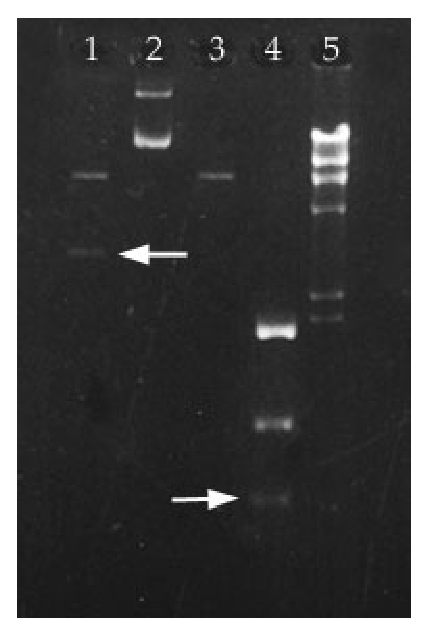
\includegraphics[height=5cm,
    angle=0]{./images/Southern-blotting.eps}}
  \caption{Example of Southern blotting}
\label{fig:Southern-blotting}
\end{figure}


{\bf HOW TO READ}: There are a few lanes, and the figure is show such taht the bigger DNA
fragments, which migrate slower, is showed as staying on top of the figure.
\begin{enumerate}
  \item lanes: 
  \begin{itemize}
    \item Standard Lanes:
    
    
    \item Sample Lanes:
    Each lane has DNA fragments restricted by a given restriction enzyme from
    one DNA sample. All these DNA samples, can be from the same stock of DNA
    digested with 3 different Restriction Enzymes, or maybe from different
    pieces of DNA altogether.
    
     When we are interested in determining the success of a particular digest,
    we often want to calculate the size of these bands, which we need to
    reference to Standard Lanes.
  \end{itemize}
  
  \item as the total DNA amounts are the same in each lane, 
  at one location, the band in one lane can be brighter than that in another
  lane. On a molar level, much more DNA of one size is present in that band than
  in a different band, although the lesser amount may be a larger fragment.
  
  
\end{enumerate}
\url{http://www.life.illinois.edu/molbio/geldigest/photo.html}



 
  There are often 3 lanes: left lanes are for DNA ladder, middle lane for the
  DNA fragments of interest, the right lane is also for DNA ladder.
  In this case, left lane and right lane are Standard Lanes, or sometimes
  Molecular Weight Markers or "Ladders". They are similar to the Control in an
  experiment, because we know exactly how they are going to turn out every time.
  These lanes contain DNA of a specific, predetermined size from a known source,
  digested with a Restriction Enzyme that cuts that piece of DNA a known number
  of times, yielding a predicted number of bands whose size we know exactly.
  
  
  To help identify the molecular weight (M.W.) along the axis, DNA ladder
  are often provided, DNA ladders are those with known molecular weights, and their
  migration along the matrix can be used as a reference to identify the M.W. of
  the DNA fragments of interest on the middle lane.
  PRINCIPLE: molecular weight is inversely proportional to migration rate through a gel
  matrix via alogarithmic relationship.
  \url{https://en.wikipedia.org/wiki/Molecular-weight_size_marker}
  
  One important sample every experiment should include is uncut DNA. Uncut DNA
  exists in as many as three different forms: {\bf supercoiled, relaxed
  circular, and linear}. Just because you didn't add any RE to your sample does
  not mean it hasn't gotten nicked or even cut at some point in its preparation. Nicking
  causes supercoiling to be relaxed, while cutting as you know causes
  linearization. Nothing has been removed from this piece of DNA, so all 3 forms
  are the same size. Does that mean they will migrate the same? Unfortunately
  no. Imagine a rubber band all twisted up into a little knot. That is very much
  like the compact form of supercoiled DNA. The relaxed, unknotted rubber band
  is similar to the circular form, and if you were to cut the rubber band once
  with scissors, it would resemble linear DNA. Which will experience the most
  resistence in an agarose gel? The least? From fastest to slowest is
  supercoiled, circular, then linear, despite the fact that all three fragments
  are of exactly the same length.
  
  

\subsection{Northern blotting (i.e. detect RNA, mRNA)}
\label{sec:Northern-blotting}

Northern blotting was developed by Alwine and his colleagues in 1979.
The name was chosen as a misnomer to 'Southern'.

The differences with Southern blotting are
\begin{itemize}
  \item detect RNA (not DNA), i.e. level of density implies the number of RNA
  molecules.

The intact mRNA molecules purified from mutant and control liver cells are
fractionated on the basis of their sizes into a series of bands by gel
electrophoresis. 

  
  \item use a different filter, i.e. Amino benzyloxymethyl filter
  
  \item RNA-(DNA probe) hybridization, rathern than DNA-(DNA probe)

Then, to make the RNA molecules accessible to DNA probes, a replica of the
pattern of RNA bands on the gel is made by transferring ("blotting") the
fractionated RNA molecules onto a sheet of nitrocellulose or nylon paper. The
paper is then incubated in a solution containing a labeled DNA probe whose
sequence corresponds to part of the template strand that produces albumin
mRNA. The RNA molecules that hybridize to the labeled DNA probe on the paper
(because they are complementary to part of the normal albumin gene sequence)
are then located by detecting the bound probe by autoradiography or by
chemical means.

The size of the RNA molecules in each band that binds the probe can be
determined by reference to bands of RNA molecules of known sizes (RNA standards)
that are electrophoresed side by side with the experimental sample.



\end{itemize}

Newer methods to detect RNA level:  RT-PCR (Sect.\ref{sec:RT-PCR}), gene array
analysis and nuclease protection assays.

\subsection{FISH technique (i.e. detect mRNA)}
\label{sec:FISH}

Detecting intracellular features such as specific mRNA molecules does not
require antibodies and possesses enormous potential because it can exploit the
genomics and microarray data, i.e.  single cell mRNA abundance measurements are
required. 

Count individual mRNAs within single cells using  florescent in-situ
hybridization (FISH) techniques has some limitation:  (1) require optimized cell
fixation protocols that are not universally applicable to all tissues and cell
types; (2)  tens of probes per RNA molecule need to be designed to generate a
detectable signal.

A better technique is RT-PCR - Sect.\ref{sec:RT-PCR}.

\subsection{PCR - polymerase chain reaction}
\label{sec:PCR}

Now that so many genome sequences are available, genes can be cloned directly
without the need to construct DNA libraries first. A technique called the
polymerase chain reaction (PCR) makes this rapid cloning possible 

PCR allows the DNA from a selected region of a genome to be amplified a
billionfold, effectively "purifying" this DNA away from the remainder of the genome.
\begin{itemize}
  \item a region of DNA fragment to be 'amlified' is separated using heat
  
  \item the desired DNA oligonuleotides as primers attach to each side to start
  the {\it in vitro} DNA synthesis (with the help of DNA polymerase)
  
  \item the process in step 2 is then repeated as many time as you want (using
  as many cloned copies present as the sources); eventually billion copies of
  the DNA fragments are generated.
  
  After three more cycles, 240 of the 256 DNA chains correspond exactly to the
  original bracketed sequence, and after several more cycles, essentially all of
  the DNA strands have this unique length. 
\end{itemize}

The PCR method is extremely sensitive; it can detect a single DNA molecule in a
sample. Trace amounts of RNA can be analyzed in the same way by first
transcribing them into DNA with reverse transcriptase - Sect.\ref{sec:RT-PCR}).

The PCR cloning technique has largely replaced Southern blotting
(Sect.\ref{sec:Southern-blotting}).

\subsection{RT-PCR, scRT-PCR (i.e. detect mRNA)}
\label{sec:RT-PCR}
\label{sec:scRT-PCR}

Single-cell {\bf reverse transcription polymerase chain reaction} (RT-PCR or
scRT-PCR) is a novel technique to count mRNA based on PCR (Sect.\ref{sec:PCR}).
It is a much simpler technique for mRNA quantification that has a large dynamic
range and is amenable to high kkthroughput analysis (Raj and Oudennarden 2009,
Dimov et al., 2014).

Single-cell RT-PCR (scRT-PCR) verification is often used in combine with
patch-clamp - Sect.\ref{sec:patch-clamp-whole-cell}.

% reverse transcription-PCR (scRT-PCR) and
% patch-clamp studies (Johns et al., 1997; Dryer et al., 1998; Martina et al.,
% 1998).

\section{-------------------}
\label{sec:techniques-clone-DNA}

Any DNA fragment that contains a gene of interest can be cloned. DNA cloning has
2 meanings
\begin{enumerate}
  \item isolation of a particular stretch of DNA (often a particular gene) from
  the rest of a cell's DNA.

  \item making many identical copies of a DNA molecule - This can be done simply
  by inserting a particular fragment of DNA into the purified DNA genome of a
  self-replicating genetic element-generally a virus or a plasmid.

The techniques to alter isolated gene and transferred back into the
germ line of an animal or plant, so as to become a functional and heritable part
of the organism's genome. 

The principles underlying the methods used for cloning genes are the same for
either type of cloning vector, although the details may differ. Today most
cloning is performed with plasmid vectors.

Plasmid (vector) - circular DNA that can replicate independently of the genome.
Plasmids were used to clone fragments of DNA of 1,000 to 30,000 nucleotide
pairs. 
\begin{enumerate}
  \item PAC
  \item BAC
  
New {\bf plasmid vectors} from bacteria based on the naturally occurring F
plasmid of E. coli can clone fragments of DNA of 100,000-300,000 nucleotide
pairs. F-plasmid and its derivative, the bacterial artificial chromosome (BAC) -
is present in only one or two copies per E. coli cell.

  \item YAC - Sect.\ref{sec:YAC} such as pYAC3, pYAC4 plasmids.
  
  For very larger DNA fragments (up to 2 Mbp), YAC is used.
  
\end{enumerate}
\end{enumerate}

\begin{figure}[htb]
  \centerline{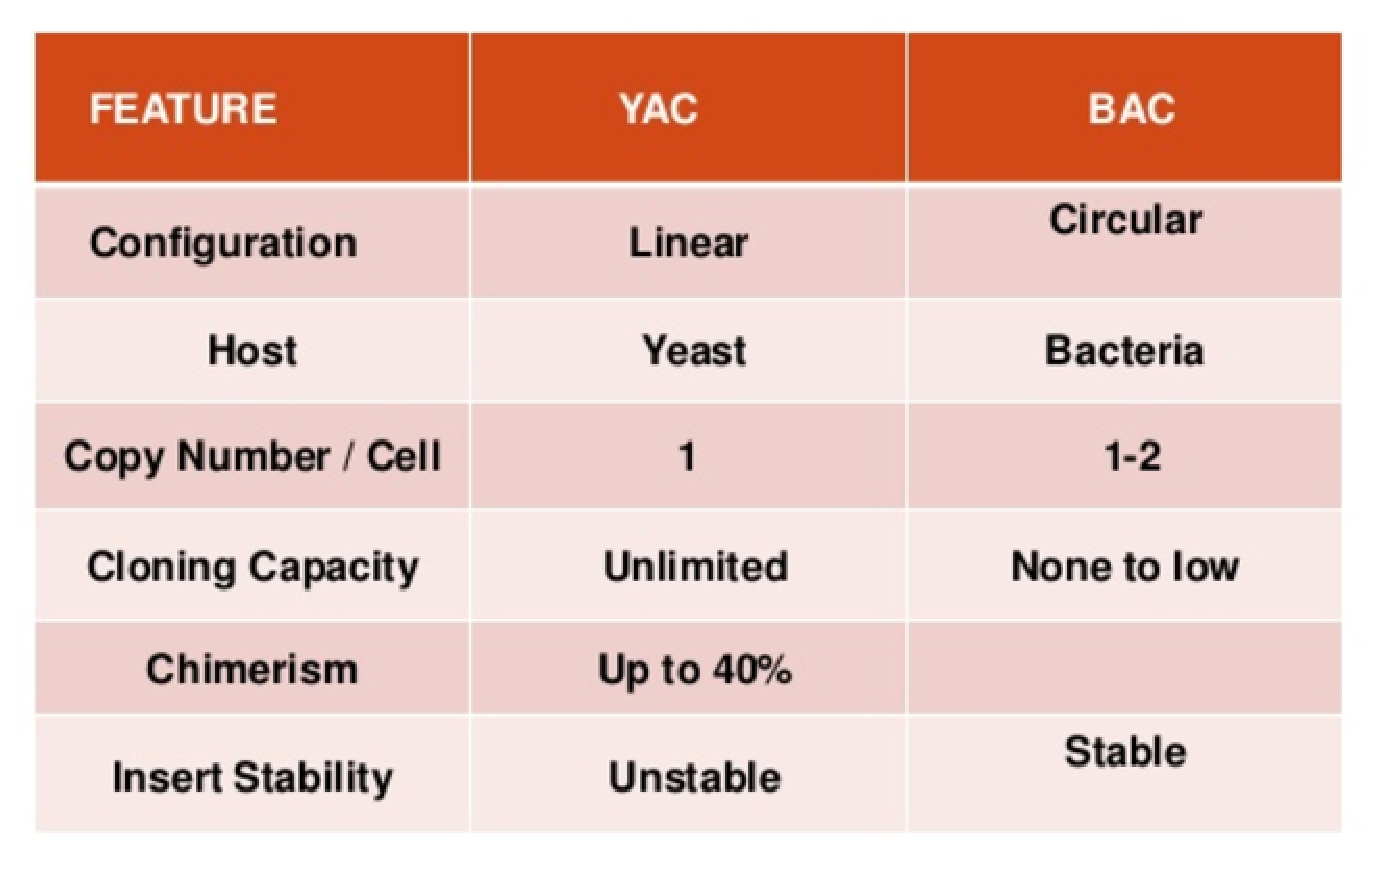
\includegraphics[height=4cm]{./images/YAC-BAC.eps}}
  \caption{Compare YAC and BAC}\label{fig:YAC-BAC}
\end{figure}


\section{P1 artificial chromosomes (PACs)}
\label{sec:PAC}

\section{Bacterial Artificial Chromosome (BAC)}
\label{sec:BAC}
\label{sec:plasmid-vector}

To study human genome, which is too big, to be able to sequence from one end to
the other; they are broken down into manageable chunks. The DNA from white blood
cells are often being used. Fragments of human DNA are then stored in bacteria,
e.g. {\it E. Coli}, from which it can be sequenced and cloned.

A {\bf plasmid} is a genetic structure, i.e. typically in the form of a circular DNA
strand in the cytoplasm of the bacterium or protozan, that can replicate itself
independently of the chromosomes. 

{\bf F plasmid} present in only one or two copies per E. coli cell.
The low number reduces the chance for  the cloned DNA fragments to become
scrambled due to recombination with sequences carried on other copies of the
plasmid. This enhances the stability to clone large DNA fragments.

Bacterial Artificial Chromosome (BAC) refers to the technique to insert a DNA
fragment into a bacterial cell (e.g. E.Coli) using a plasmid called {\bf BAC
vector}. An E.coli genome is about 3 Mbp and you can't put much more than
200-300Kbp without stunting its growth (and favoring the growth of
recombinants). So, a {\bf BAC vector} can hold a DNA fragment of up to 300 kb.

The BAC vector, now with the foreigner DNA fragment, is then transfered to the
bacteria, which then can mobilize from F+ male bacteria to F- female bacteria.
{\bf Conjugation} is the gene that transfers from one bacteria to another.

The structure of a BAC vector
\begin{enumerate}
  \item  a cloning site (which can splitted to accept the DNA fragment): include
  {\it lacZ}
  
  \item F plasmid {\it par genes} (F = fertility)
  
  F factor controls its own replication, with two origins of replication: {\bf
  oriV} (for bidirectional replication) and {\bf oriS} (for unidirectional
  replication). It also has a genes that regulate DNA synthesis to keep its copy
  at a low level; and a gene that regulates the partition into daughter cells
  after {\it E. Coli} divides.
  
  \item ori
  
  \item Cm$^R$
\end{enumerate} 

BACs are preferred over YACs (Sect.\ref{sec:YAC}) because growing yeast and
purifying YACs is much more difficult compared to growing E. coli and purifying
BACs.  Finally, the entire BAC clones can be shotgun-sequenced fairly rapidly
(Sect.\ref{sec:shotgun-sequencing-method}).

\section{Yeast Artificial Chromosome (YAC)}
\label{sec:YAC}


Yeast artificial chromosomes (YACs) are genetically engineered chromosomes (i.e.
synthetic chromosome) derived from the DNA of the yeast, Saccharomyces
cerevisiae, to contains a targeted DNA fragment from another species. 
It has
\begin{enumerate}
  \item centromere
  \item telomere
  \item autonomous replicating sequence (ARS) element - required for
  replication and preservation of YAC in yeast cells
\end{enumerate}

YAC was first described in 1983 by Murray and Szotak.
YAC can behave like naturally existing chromosomes, provided they have proper
size. Different YAC plasmids: pYAC3, pYAC4 plasmids, Fig.\ref{fig:YAC-pYAC3}.

\begin{figure}[htb]
  \centerline{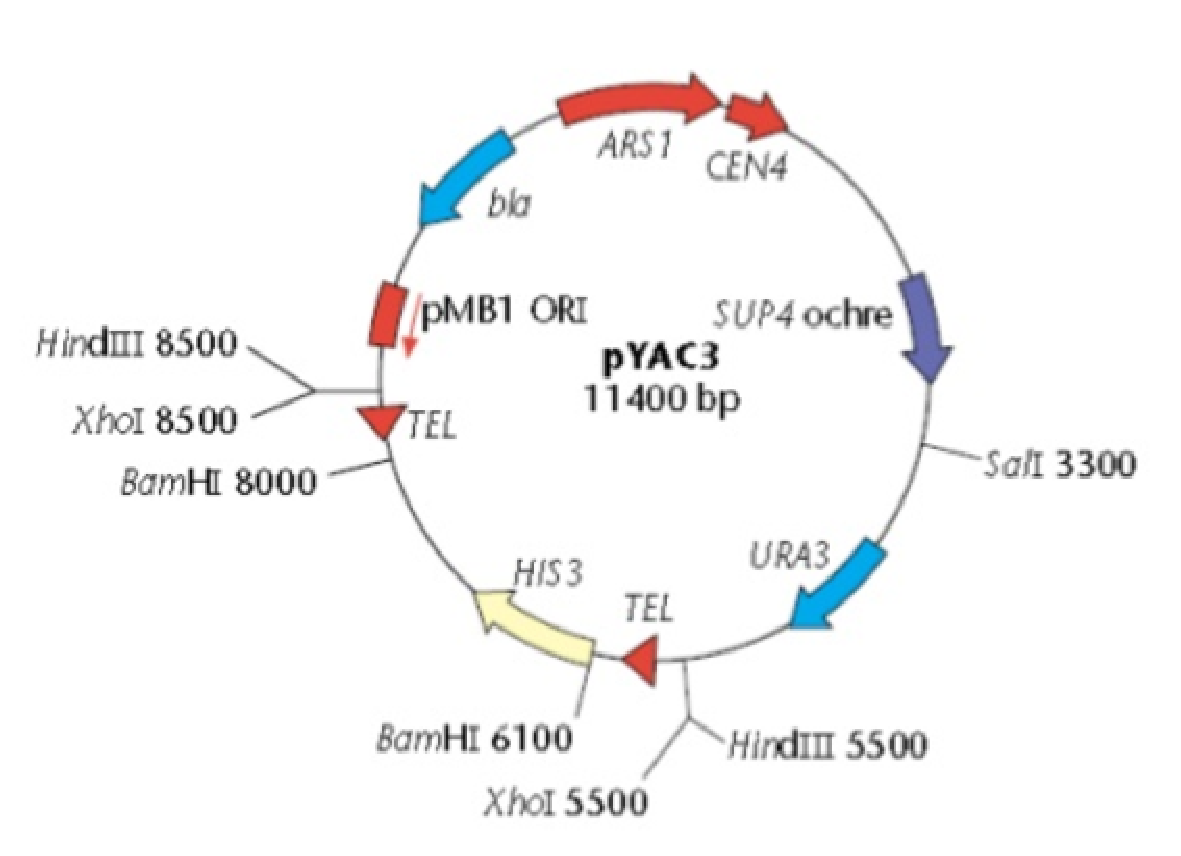
\includegraphics[height=3cm]{./images/YAC-pYAC3.eps}}
  \caption{pYAC3}\label{fig:YAC-pYAC3}
\end{figure}

YAC (to contain a foreigner DNA) is built using an initial circular plasmid,
Fig.\ref{fig:YAC-pYAC3}, and then typically broken into 2 linear molecules using
restriction enzymes; before a DNA ligase is used to ligate a sequence or gene of
interest between 2 linear molecules. YAC can contain more base pairs (up to
2 Mbp) than BAC's F-plasmid vectors (Sect.\ref{sec:BAC}), i.e.
100-1000 kb (i.e. over a million base pairs). However, YACs are significantly
less stable than BACs.s

{\bf Examples of yeast expression vectors}: YACs, YIps (yeast integrating
plasmids), and YEps (yeast episomal plasmids). A YAC is a circular DNA plasmid
where the target DNA fragment can be inserted, before being inserted into the
yeast.


 
 
\section{-------------------}
 
\section{DNA libraries}
\label{sec:DNA-libraries}

A DNA library is a comprehensive collection of cloned DNA fragments from a cell,
tissue, or organism. 

This library includes (one hopes) at least one fragment that contains the gene
of interest. Libraries can be constructed with either a virus or a plasmid
vector (Sect.\ref{sec:techniques-clone-DNA}) and are generally housed in a
population of bacterial cells. 

BACs (Sect.\ref{sec:BAC}) are now the preferred vector for building DNA
libraries of complex organisms - including those representing the human and
mouse genomes.

\subsection{traditional methods}

Sequencing the DNA directly from DNA fragments limit the amount of genes can be
detected. A better method is building cDNA libraries -
Sect.\ref{sec:cDNA-libraries}.
\begin{verbatim}
DNA ---[DNA restriction nuclease]---> DNA fragments (double-strand)
                                    (some with full-genes; many not)
                                    
          DNA fragments ---[inserted into plasmid vectors]---> vector
          
          vector  --[cloning]-->  DNA cloning
\end{verbatim}

IMPORTANT: As the genomic DNA is cut into fragments at random, only some
fragments contain genes. Many of the genomic DNA clones obtained from the DNA of
a higher eucaryotic cell contain only noncoding DNA


\subsection{cDNA libraries}
\label{sec:cDNA-libraries}

An alternative strategy is to begin the cloning process by selecting only those
DNA sequences that are transcribed into mRNA and thus are presumed to correspond
to protein-encoding genes. 

\begin{verbatim}
DNA --[transcription]-> RNA transcripts --> mRNA 
         mRNA --[reverse transcription]---> (complement) DNA single-strand

         cDNA --[DNA polymerase]---> DNA-containing gene double-strand
         
         DNA double-strand --[inserted into plasmid vector]--> vector

         vector  --[cloning]-->  DNA cloning
\end{verbatim}

This is done by extracting the mRNA (or a purified subfraction of the mRNA) from
cells and then making a complementary DNA (cDNA) copy of each mRNA molecule
present; this reaction is catalyzed by the reverse transcriptase enzyme of
retroviruses, which synthesizes a DNA chain on an RNA template. 

The single-stranded DNA molecules synthesized by the reverse transcriptase are
converted into double-stranded DNA molecules by DNA polymerase, and these
molecules are inserted into a plasmid or virus vector and cloned.
Each clone obtained in this way is called a cDNA clone, and the entire
collection of clones derived from one mRNA preparation constitutes a cDNA
library.

ADVANTAGES:
\begin{enumerate}
  \item contain the uninterrupted coding sequence of a gene.  

  \item  some proteins are produced in very large quantities by specialized
  cells. 
  
  In this case, the mRNA encoding the protein is likely to be produced in
  such large quantities that a cDNA library prepared from the cells is highly
  enriched for the cDNA molecules encoding the protein, greatly reducing the
  problem of identifying the desired clone in the library   
  
\end{enumerate}

\section{DNA sequencing}
\label{sec:DNA-sequencing}

In the late 1970s methods were developed that allowed the nucleotide sequence of
any purified DNA fragment (Sect.\ref{sec:DNA-libraries}) to be determined simply
and quickly.

Although the same basic method is still used today, many improvements have been
made. Now it is done completely automated using machines: robotic devices mix
the reagents and then load, run, and read the order of the nucleotide bases from
the gel.

The computer screen display the 'probability' that a given nucleotide (A, T, G,
C) is detected at each location, Fig.\ref{fig:DNA-sequencing}.

\begin{figure}[htb]
  \centerline{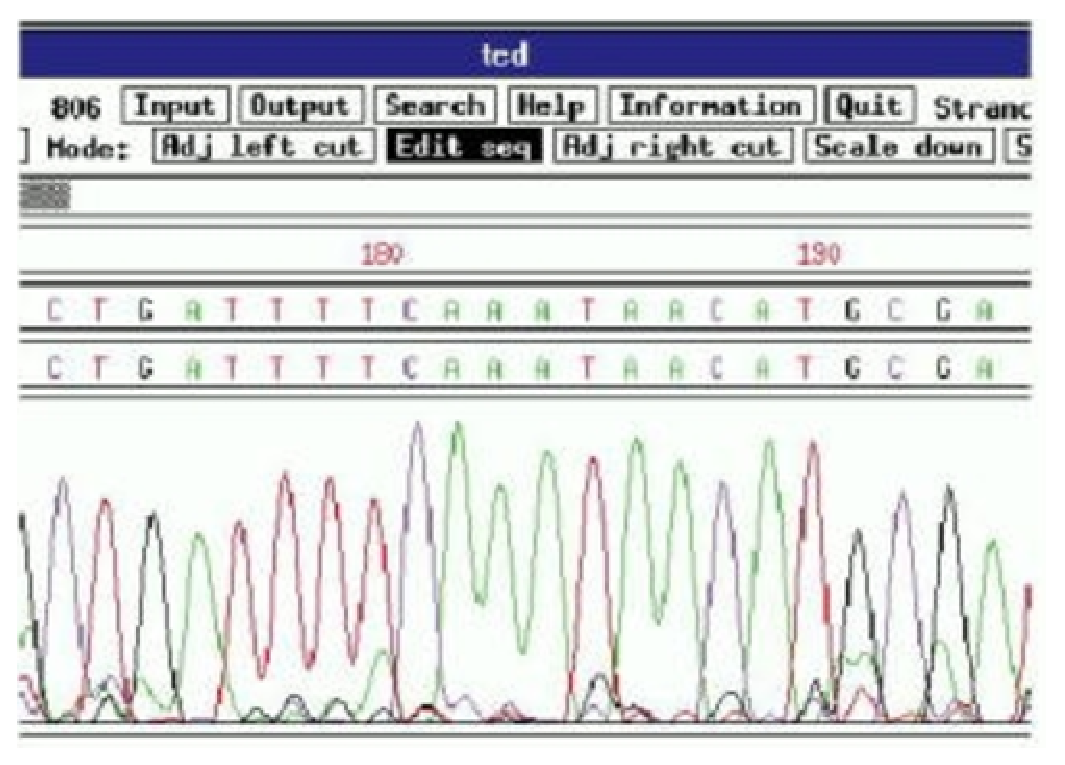
\includegraphics[height=4cm]{./images/DNA-sequencing.eps}}
  \caption{a clear stretch of nucleotide sequence can be read here between positions 173
and 194 from the start of the sequence. Each colored peak represents a
nucleotide in the DNA sequence. The figure is part of the
sequence of the genome of the plant Arabidopsis. (Courtesy of George Murphy.)}
\label{fig:DNA-sequencing}
\end{figure}

\subsection{Shotgun sequencing method}
\label{sec:shotgun-sequencing-method}

Haemophilus influenzae (a bacterium that can cause ear infections or meningitis
in children) was the first organism to have its complete genome sequence - all
1.8 million nucleotides - determined by the shotgun sequencing method, the most
common strategy used today.

In the shotgun method, long sequences of DNA are broken apart randomly into many
shorter fragments. Each fragment is then sequenced and a computer is used to
order these pieces into a whole chromosome or genome, using sequence overlap to
guide the assembly. The shotgun method is the technique of choice for sequencing
small genomes. 

Although larger, more repetitive genome sequences are more tricky to assemble,
the shotgun method has been useful for sequencing the genomes of Drosophila
melanogaster, mouse, and human.


\subsection{Nucleotide Sequences Are Used to Predict the Amino Acid Sequences of Proteins}

Although in principle there are six different reading frames in which a DNA
sequence can be translated into protein (three on each strand), the correct one
is generally recognizable as the only one lacking frequent stop codons
\begin{verbatim}
3 choices of starting point on each strand:
ABCABC
 BCABCA
  CABCAB
\end{verbatim}

If necessary, a limited amount of amino acid sequence can then be determined
from the purified protein to confirm the sequence predicted from the DNA.

The problem comes, however, in determining which nucleotide sequences-within a
whole genome sequence-represent genes that encode proteins. 
\begin{enumerate}
  \item  It is easier if DNA sequence from a bacterial or archeal chromosome,
  which lacks introns, or from a cDNA clone.
  
  The location of genes in these nucleotide sequences can be predicted by
  examining the DNA for certain distinctive features:
  by searching the nucleotide sequence for open reading frames (ORFs) that begin
  with an initiation codon, usually ATG, and end with a termination codon, TAA,
  TAG, or TGA.
  
  To minimize errors, computers used to search for ORFs are often directed to
  count as genes only those sequences that are longer than, say, 100 codons in
  length. 
  
  
  \item   more complex genomes, such as those of eucaryotes, the process is
  complicated by the presence of large introns embedded within the coding
  portion of genes. 
  
  In many multicellular organisms, including humans, the average exon is only
  150 nucleotides long.
  
  To deal with this, a second major approach to identifying the coding regions
  in chromosomes is through the characterization of the nucleotide sequences of
  the detectable mRNAs (in the form of cDNAs). The mRNAs (and the cDNAs produced
  from them) lack introns, regulatory DNA sequences, and the nonessential
  "spacer" DNA that lies between genes. It is therefore useful to sequence large
  numbers of cDNAs to produce a very large collection (called a database) of the
  coding sequences of an organism.
\end{enumerate}

{\bf Predicting}: For nucleotide sequences that are conserved between closely
related organisms usually encode proteins, comparison of these conserved
sequences in different species can also provide insight into the function of a
particular protein or gene.

\subsection{why genome sequencing?}

This is part of the emerging field {\bf genomics}.
The genomes of many organisms have been fully sequenced; these include plant
chloroplasts and animal mitochondria, large numbers of bacteria and archea, and
many of the model organisms that are studied routinely in the laboratory,
including several yeasts, a nematode worm, the fruit fly Drosophila, the model
plant Arabidopsis, the mouse, and, last but not least, humans.   


Researchers have also deduced the complete DNA sequences for a wide variety of
human pathogens. These include the bacteria that cause cholera, tuberculosis,
syphilis, gonorrhea, Lyme disease, and stomach ulcers, as well as hundreds of
viruses-including smallpox virus and Epstein-Barr virus (which causes infectious
mononucleosis).

Examination of the genomes of these pathogens should provide clues about what
makes them virulent, and will also point the way to new and more effective treatments.

Comparison of the complete genome sequences of different organisms allows us to
trace the evolutionary relationships among genes and organisms, and to discover
genes and predict their functions.

Assigning functions to genes often involves comparing their sequences with
related sequences from model organisms that have been well characterized in the
laboratory, such as the bacterium E. coli, the yeasts S. cerevisiae and S.
pombe, the nematode worm C. elegans, and the fruit fly Drosophila.

{\bf LIMITATION}: although comparative analysis of genomes reveals a great deal
of information about the relationships between genes and organisms, it often
does not provide immediate information about how these genes function, or what
roles they have in the physiology of an organism, i.e. in the context of a
living organism.


\section{Antibody}
\label{sec:antibody}



Antobodies actually include several classes of molecules
\begin{enumerate}
  \item {\bf IgG}: (most useful)  a protein molecule that is made and secreted
  and can recognize specific antigens.
  
  \item {\bf IgM}: designed to be expressed on the cell surface
  
  \item {\bf IgA}: designed for secretion in the bodily fluids 
\end{enumerate}

Antibodies are often used to help detecting an antigen (Sect.\ref{sec:antigen}),
using one of the following techniques
\begin{enumerate}
  \item Western blot - Sect.\ref{sec:Western-blot}
  
  \item Immunohistochemistry (IHC) - Sect.\ref{sec:immunohistochemistry}
\end{enumerate}
\url{http://www-users.med.cornell.edu/~jawagne/Antibody_Approaches.html}

As a single antibody only target a specific segment of the antigen, to ensure
the protein is full-length, not a fragment, it is often better to 
utilize several antibodies that spanned the entire length of the HTT protein,
e.g. antibodies for detecting Htt protein (Hughes, Jones, 2011).





\subsection{IgG}
\label{sec:IgG-antibody}

IgG is composed of two subunits including two "heavy" chains and two "light"
chains

\subsection{Immunohistochemistry (IHC)}
\label{sec:immunohistochemistry}

IHC method elucidate tissue-specific and subcellular localization of an antigen
within a sample.  IHC staining is accomplished using antibodies that recognize a
target protein and antibody-antigen complexes that are visualized via
chromogenic, radioactive or fluorescent substrates.

The method is less quantitative than western blot
(Sect.\ref{sec:Western-blot}) or ELISA (Sect.\ref{sec:ELISA}), yet they offer
the advantage of characterizing protein expression in the context of intact
tissue.

\subsection{Enzyme-linked immunosorbent assay (ELISA)}
\label{sec:ELISA}


\url{http://www.abcam.com/protocols/antibody-methods-and-techniques}

\subsection{Immunocytochemistry (ICC)}
\label{sec:ICC}
\label{sec:immunocytochemistry}

ICC is used to study the subcellular distribution of proteins using
fluorescently-labeled antibodies.

In contrast with IHC, this technique affords {\it greater spatial resolution} as
cultured cells lack the complex surrounding environment found in tissue samples.

\subsection{Flow cytometry}
\label{sec:Flow-cytometry}
\label{sec:flow-cytometry}

{\bf Flow cytometry} has been primarily used to address single-cell behavior. 
Flow cytometry is a means of measuring certain chemical and physical properties
of cells. Parameters measure include {\bf cell-size} and the expression of
cell-surface and intracellular markers. 

Flow cytometry measures the fluorescence emitted by labeled antibodies, bound to
individual cells in a mixed population.

While flow cytometry is effective, it is limited by the availability of
antibodies. Only a minority of known human genes have commercially available
antibodies. {\it Flow cytometry is also difficult to perform when the
distinguishing features of subpopulations are molecules inside the cells rather
than on the surface of cells.}

Recently, a tool employing mass spectrometry has been developed to leverage the
precision of flow cytometry analysis. The combination of the two techniques,
termed single-cell mass cytometry (CyTOF), allows the simultaneous measurement
of more than 40 cellular parameters at single-cell resolution with over 100
available detection channels (Janes et al., 2011; Spitzer et al, 2016).
% Janes, M. R. & Rommel, C. Next-generation flow cytometry. Nat. Biotechnol. 29,
% 602-604 (2011).
% Spitzer, M. H. & Nolan, G. P. Mass cytometry: single cells, many features. Cell
% 165, 780-791 (2016).  

Compared to fluorescence-based cytometry, mass cytometry employs element-tagged
probes that enable the discrimination of elements according to their mass/charge
ratio (m/z), with minimal overlap and background cellular signal. All these
attributes simplify the large panel experimental design, thus uniquely enabling
high-dimensional cytometry experiments that would not be possible otherwise



\subsection{Fluorescence-activated cell sorting (FACS)}
\label{sec:FACS}

Fluorescence-activated cell sorting (FACS) is a more sophisticated system,
which quantifies the fluorescent signal and separates the cells from a mixed
population that contains preselected characteristics (i.e. fluorescence
intensity, size and viability).  

\subsection{Immunoprecipitation (IP)}
\label{sec:Immunoprecipitation}

Immunoprecipitation is a versatile technique that enables isolation and
purification of individual and complexed proteins.
Antibodies are immobilized on solid-phase substrates (e.g. magnetic/agarose
beads), which capture antigens from complex solutions.

\subsection{Chromatin immunoprecipitation (ChIP)}
\label{sec:ChIP}

Chromatin immunoprecipitation (ChIP) is a procedure used to determine whether a
given protein binds to a specific DNA sequence in vivo.


\subsection{ELISPOT}
\label{sec:ELISPOT}

ELISPOT is used for the detection of secreted proteins, such as cytokines and
growth factors. The technique enables quantification and comparison of immune
responses to various stimuli. 



\subsection{Western blot}
\label{sec:Western-blot}

It is also possible to use an antibody to detect a protein after fractionation
by SDS-PAGE, using the method called {\bf Western blotting}.

The name is chosen as the method is for fragment detection, which is analogous
with northern blotting (Sect.\ref{sec:Northern-blotting}) and Southern blotting
(Sect.\ref{sec:Southern-blotting})


\subsection{Antigen (epitope), anti-idioptype antibody}
\label{sec:antigen}
\label{sec:epitope}

An {\bf antigen} is a  protein that can be recognized (bound) by the antibody
(Sect.\ref{sec:antibody}). These antigens are most commonly polypeptides or
carbohydrates, but they can also be lipids, nucleic acids, or even small
molecules like neurotransmitters. 

A particular antibody molecule can only interact with a small region of an
antigen (called {\bf epitope}) and in the case of a polypeptide this is
generally about 5-12 amino acids. This region can be continuous or it can be
distributed in different regions of a primary structure that are brought
together because of the secondary or tertiary structure of the antigen.

{\it It is possible, although unlikely, that the same, or closely related
epitopes, could be shared by the different antigens.}

In some cases, it is possible to make an antibody that is directed {\bf against}
the antigen binding site of another antibody. This type of antibody is called an
{\bf anti-idiotype antibody}.

\section{ membrane-selective FM-dyes}
\label{sec:FM-dyes-membrane-selective}

The membrane-selective FM-dyes, FM4-64 and FM1-43, belong to a class of
amphiphilic styryl dyes developed by Betz and co-worker (Betz et al., 1992,
1996) which are both membrane-selective fluorescent dyes. The abbreviation 'FM'
stands for the chemist's name, Fei Mao, who developed the FM-dyes from the
related probe, dimethylaminostyrylmethylpyridiniumiodine (DASPMI).
 
FM-dyes fluoresce significantly only when they are in a hydrophobic
environment, e.g. a lipid-rich membrane.

FM4-64 and FM1-43 differ slightly in their chemical structure, and these
structural differences can result in different patterns of membrane staining
(Fischer-Parton et al., 2000; Hickey et al., 2002).  


\subsection{FM4-64 dye}
\label{sec:FM4-64-dye}

Styryl dye FM 4-64 has been reported to selectively stain yeast vacuolar
membranes with red fluorescence (excitation/emission maxima ~515/640 nm). 
FM4-64 is usually preferred to FM1-43 due to its superior brightness, greater
contrast, higher photostability, and its red-shifted emission facilitating
concomitant use with the green fluorescent protein (GFP) (Bolte et al., 2004).

This lipophilic dye is an important tool for visualizing vacuolar organelle
morphology and dynamics, for studying the endocytic pathway and for screening
and characterizing yeast endocytosis mutants. 

\chapter{Software and Database of organic compounds (e.g. proteins)}



\section{Organic compound databases}
\label{sec:databases}


\begin{itemize}
\item	{\bf CAS database} is the most comprehensive repository for data
  on organic compounds. The search tool SciFinder is offered.

\item {\bf Beilstein database} contains information on 9.8 million
  substances, covers the scientific literature from 1771 to the
  present, and is today accessible via CrossFire. 
  
  Structures and a large diversity of physical and chemical properties is
  available for each substance, with reference to original literature.

\item {\bf PubChem database} contains 18.4 million entries on compounds and
especially covers the field of medicinal chemistry.
\end{itemize}


\section{Software tools}
\label{sec:tools}

As the 3D structure of a biomolecule define its function, it is important to
understand/predict the 3D structure. We discuss software tools for visualizing
the 3D structure of biomolecules (Sect.\ref{sec:living-organisms}).

\subsection{MDLChime}
\label{sec:MDLChime}

It is recommended to use Jmol (Sect.\ref{sec:Jmol}) instead.

If you still want to use MDLChime, check the link \url{http://www2.mdl.com/}.
MDLChime provide capability to
\begin{itemize}

   \item view and manipulate PDB file (the file that contains information which
can be used to generate 3D structure of proteins) and other molecular models
via the web browser (i.e. directly from a WWW page)

   \item How to install MDLChime manually to run with
Firefox\footnote{\url{http://www.umass.edu/microbio/chime/pe_beta/pe/protexpl/chiminst.htm}}:

   \item Sample image to
test\footnote{\url{http://www.umass.edu/microbio/chime/atp.pdb }}
\end{itemize}

\subsection{Jmol}
\label{sec:Jmol}

Jmol is better than MDLChime (Sect.\ref{sec:MDLChime}), as it is a desktop-based
program, and has more features, e.g. RasMol scripting language
(Sect.\ref{sec:Rasmol}).

URL: \url{http://jmol.sourceforge.net/} (a replacement for MDLChime)

\subsection{Protein Explorer (PE) - Windows only)}
\label{sec:Protein-Explorer}


Protein Explorer: (best for beginners, work only in Windows, requires MDLChime browser plugin) 
\begin{itemize}
  
\item view three-dimensional structures of protein, DNA, and RNA
  macromolecules, and their interactions and binding of ligands,
  inhibitors, and drugs

\item \url{ http://www.umass.edu/microbio/chime/pe_beta/pe/protexpl/frntdoor.htm}

\item Offline tool:
\url{http://www.umass.edu/microbio/chime/regisfrm/downlpew.htm}

\end{itemize}

\subsection{MolSlide Manager}
\label{sec:MolSlide-Manager}

{\bf MolSlide Manager}: an utility that helps you create 3D molecular structure
and view it without using Protein Explorer (PE) or MDLChime, and the image can
be included in your report or tutorial
presentation\footnote{\url{http://www.umass.edu/microbio/chime/pe_beta/pe/protexpl/molview/
}}.

\subsection{Rasmol}
\label{sec:Rasmol}

Rasmol is no longer under development (last is 2009). Jmol
(Sect.\ref{sec:Jmol}) and Sirius has incorporated the RasMol scripting language
into its commands.

\url{http://alternativeto.net/software/rasmol/}



\subsection{PyMOL}
\label{sec:PyMol}

PyMOL can produce high-quality 3D images of small molecules and biological
macromolecules, such as proteins. PyMOL is one of a few open-source
visualization tools available for use in structural biology.

PyMOL uses OpenGL Extension Wrangler Library (GLEW) and Freeglut, and can solve
Poisson-Boltzmann equations using the Adaptive Poisson
Boltzmann Solver.


\begin{verbatim}
Amoeba = amip
Rotifers = a microscopic organism
Rumen = (dvat.hoc) da. co? (cu?a tra\^u,bo')
erythrocyte = red blood cell
leukocyte = white blood cell
platelet = thrombocyte = a small blood cell needed for normal blood clotting 
cerebellum = brain,
epithelial = (bie\^?u mo\^) belonging to or formed by epithelium
epithelium = a layer of cells which form or covering over the internal and external surfaces of the body

\end{verbatim}


\chapter{Biology of cell}
\label{chap:cell-life}

A cell is a unit of life (Sect.\ref{sec:incredibility-life}).

\section{Cell types and cell's organelles}
\label{sec:cell-types}
\label{sec:cell-organelles}

A cell type is a classification used to distinguish between morphologically or
phenotypically distinct cell forms within a species. Cells might look different
under a microscope, most cells have chemical and structural features in common.
In each cell, there are about {\bf 20 different types of organelles and
structures}.

Your body has many different kinds of cells. In humans, there are about {\bf 200
different types of cells} (a number which seems low given the amount of
diversity and specialization in our body).

From a single zygote, the human body grows into {\bf 37 trillion cells}. Each
cell type is derived from one of the three regions in early stage of embryonic
development (Sect.\ref{sec:brain_development}): endoderm, mesoderm and ectoderm
(Sect.\ref{sec:endoderm}).

Each cell is a complex living system, with 
\begin{itemize}
  \item a machine to produce products, i.e. different proteins
  \item the proteins are made based on the given footprint, i.e. the genetic
  information encoded in the DNA sequences which is wrapped in the molecules
  called chromosomes (Sect.\ref{sec:chromosome}), which locates
  inside the nucleus.

Even though all cells have the same genetic information, i.e. the same exact
copy of the set of chromosomes (e.g. in human is 23 set of chromosomes),
different cell types express different subset of genes at different expression
levels for each gene.

\end{itemize}


The mRNA (Sect.\ref{sec:mRNA}) present in each cell gives a snapshot of the
genes that are expressed and important to that cell. Different types need to
express different genes and so accumulate different mRNAs. It's far easier to
measure a cell's mRNA than, say, its protein levels, because we are very skilled
at analyzing at amino-acid sequences.
\footnote{\url{http://www.nature.com/scitable/blog/bio2.0/discovering_new_cell_types_one}}


Link:
\url{https://en.wikipedia.org/wiki/List_of_distinct_cell_types_in_the_adult_human_body}


\section{Cell culture}
\label{sec:cell-culture}

Cell culture is the process by which cells are grown under controlled
conditions, generally outside of their natural environment.

\section{Cell line}
\label{sec:cell-line}

A cell line refers to a population of cell culture (Sect.\ref{sec:cell-culture}) developed from a single cell and
therefore consisting of cells with a uniform genetic makeup.
\begin{enumerate}
  \item first: separate single cell

Cells can be isolated from tissues for ex vivo culture in several ways.
  
  \item second: grow the cell: only the white cells are capable of growth in
  culture.
  
Cells are grown and maintained at an appropriate temperature and gas mixture
(typically, 37$^\circ$C, 5\% CO2 for mammalian cells) in a cell incubator.
Aside from temperature and gas mixture, the most commonly varied factor in
culture systems is the cell growth medium. Recipes for growth media can vary in
pH, glucose concentration, growth factors, and the presence of other nutrients.

\end{enumerate}
\url{https://en.wikipedia.org/wiki/Cell_culture}

\subsection{Immortalized cell line}

A typicall cell would normally not proliferate indefinitely (the division stops
after a number of cell divisions) but for some cell (such as HeLa cell -
Sect.\ref{sec:HeLa-cell-line}), due to mutation, have evaded normal cellular
senescence and instead can keep undergoing division. Such cell line is called
{\bf immortalized cell line}.
An immortalised cell line should not be confused with stem cells, which can also
divide indefinitely, but form a normal part of the development of a
multicellular organism.

Researchers have identified numerous ways to transform primary tissues from
humans and animals into immortalized cell lines.
There are various immortal cell lines. 
\begin{itemize}
  \item Some of them are normal cell lines - e.g. derived from stem cells. 

   \item Other immortalised cell lines are the in vitro equivalent of cancerous
   cells.

Cancer occurs when a somatic cell which normally cannot divide undergoes
mutations which cause de-regulation of the normal cell cycle controls leading to
uncontrolled proliferation. Immortalised cell lines have undergone similar
mutations allowing a cell type which would normally not be able to divide to be
proliferated in vitro.

\end{itemize}

Embryonic and induced pluripotent stem cells
(Sect.\ref{sec:induced-pluripotenti-stem-cell-line}) may get more media
attention, but ordinary somatic cell lines still form the backbone of biomedical
research.


 
\subsection{-- HeLa cell line}
\label{sec:HeLa-cell-line}
\label{sec:cell-line-HeLa}

On February 8, 1951, George Gey of Johns Hopkins University isolated some cells
from a cervical cancer biopsy (from the patient named Henrietta Lacks) and
placed them into a petri dish with some medium.

Lacks died of her cancer eight months later, but her cells, dubbed {\bf HeLa},
became the first immortalized cell line, capable of renewing itself in
artificial culture indefinitely.
In the decades since their isolation, scientists have grown an estimated 20
tons of them.
\footnote{\url{http://www.nature.com/news/most-popular-human-cell-in-science-gets-sequenced-1.12609}}

The genome of HeLa cell was sequence in 2013; however its genome is a bizarre,
error-filled genome, with one or more (with up to five copies of some) extra
copies of many chromosomes. Many genes were duplicated even more extensively,
with four, five or six copies sometimes present, instead of the usual two. 
Furthermore, large segments of chromosome 11 and several other chromosomes were
reshuffled like a deck of cards, drastically altering the arrangement of the
genes.  Around 2000 genes are expressed at levels higher than those of normal
human tissues because of the duplications.

Having been replicating in labs around the world for six decades, HeLa cells
have also accrued errors not present in the original tumour DNA.  It means it is
difficult to trace the origin of these alterations.

HeLa cells could prove useful for studying aspects of the biology of cervical
tumours, such as their response to cancer drugs.
In recent years, the genomes of many cervical tumours have been sequenced, and
so it should be possible to see how these compare with the HeLa genome.

\subsection{-- Induced pluripotent stem cell line}
\label{sec:induced-pluripotenti-stem-cell-line}
\label{sec:cell-line-induced-pluripotenti-stem}

Alternative cell lines, such as induced pluripotent stem cells generated from
patient skin cells, offer a more accurate window on human biology than HeLa
cell line.



\subsection{Cell line cross-contamination}
 
About 15-20\% of the time, cells used in experiments have been misidentified or
contaminated with another cell line. Cell line cross-contamination can be a
problem for scientists working with cultured cells.

\url{https://www.sciencemag.org/custom-publishing/technology-features/art-culture-developing-cell-lines}


\section{Transcriptional regulation}
\label{sec:transcriptional-regulation}

The first step in the translation of genomic sequence  into  physiology  or 
pathophysiology  is  transcription.

Transcriptional  regulation  has  been  studied  almost  exclusively on  nucleic
acids  extracted  from  cultured cells or tissues by
\begin{itemize}
  \item Northern blot - Sect.\ref{sec:Northern-blotting}
  
  \item differential  display
  
  \item serial  analysis  of  gene expression  (SAGE) 
  
  \item  forms  of  microarray

\end{itemize}


\subsection{Transcription factors}
\label{sec:transcription-factor}

Transcription   factors   (TF's ) are proteins that regulate gene expression.
Transcriptional regulation in eukaryotes occurs within a {\bf chromatin}
setting, and is strongly influenced by the posttranslational modification of
histones, the building blocks of chromatin, such as methylation, phosphorylation
and acetylation.

An established paradigm that TFs specifically   recognize   only   relatively
short   (4-20 bp) consensus DNA motifs in that  the consensus TATA box motif
provides the specificity. However, this has been recently challenged by
different  high-throughput methods both in  vivo and in vitro.
\begin{enumerate}

  \item  Human pre-initiation complex (PIC): there is no specificity-determining
    consensus motifs for the positioning of PIC have been identified


  
  \item 
\end{enumerate}

\subsection{Gene transcription}
\label{sec:gene-transription-process}

All cells have the same genes, but not all genes are expressed in every cell at
all times. Factors regulating the timing, rate, and location of gene expression
are encoded in DNA as well, and contribute to biologic variation.

For the  information encoded in a gene to be expressed, it goes through a
multi-step
 process:
\begin{enumerate}
  \item inside the nucleus: a specialized protein attach to the DNA strand and
  make a copy of the DNA sequence in the form of a molecule called {\bf mRNA}
  
  \item mRNA is transferred to outside the nucleus
  
  \item translation step: a cellular mechinery reads the genetic instructions in
  the mRNA and synthesizes proteins.
\end{enumerate}

\textcolor{red}{\bf IMPORTANT}: mRNA does not correspond exactly to the DNA from
which it was transcribed. After transcription in the nucleus, the sequence is
processed to remove and shuffle segments. This increases the number of proteins
that can be produced from a single gene.
{\it There are only 20,000 - 25,000 genes, but more than 200,000 different types
of proteins in the human body}.

\section{Cell type (phenotype) detection techniques}

Cellular diversity of the brain is largely attributed to the spatial and
temporal heterogeneity of progenitor cells (Sect.\ref{sec:progenitor-cell}).
 
Distinguishing cell phenotype while recording 
\begin{enumerate}
  \item axonal tracing (Kawaguchi et al., 1990): has been technically difficult
  and labor intensive
  
  \item single-cell gene profiling (Surmeier et al., 1996) such as flow
  cytometry (Sect.\ref{sec:Flow-cytometry}) which is limited by the number of
  available antibodies


  \item Detecting intracellular features such as specific mRNA molecules does not
require antibodies and  possesses enormous potential because it can exploit the
genomics and microarray data, i.e.  single cell mRNA abundance measurements are
required 
  
  count individual mRNAs within single cells using
  \begin{itemize}
    \item  florescent in-situ hybridization (FISH) techniques 
    
Limitation:   (1) require optimized cell fixation protocols that are not
universally applicable to all tissues and cell types; (2)  tens of probes per
RNA molecule need to be designed to generate a detectable signal
    
    \item reverse transcription polymerase chain reaction, RT-PCR: a
    much simpler technique for mRNA quantification that has a large dynamic
    range and is amenable to high throughput analysis 
  \end{itemize}  
\end{enumerate} 
 
\section{eGFP (enhanced green fluorescent protein) reporter genes}
\label{sec:EGFP}

Transgenic mice that express enhanced green fluorescent protein (EGFP) reporter
genes in a variety of cells have been generated (Gong et al., 2003).
This can be used to map gene expression at cellular resolution.
\begin{itemize}
  \item  green fluorescent protein (GFP) is expressed under control of D1
  receptor or D2 receptor promoter regions (Gong et al., 2003; Day et al.,
  2006).

  \item D1 and D2 EGFP-positive MSNs (Day et al., 2006;  Kreitzer and
  Malenka, 2007; Cepeda et al., 2008)

\end{itemize}


Visualization of EGFP expression in specific neuronal or glial cell populations
has also provided compelling evidence that this strategy can result in the
identification of expressing cell types, as the detailed morphology of
EGFP-expressing cells is aparent.

The endogenous messenger RNA and protein coding sequences have been replaced by
sequences encoding the EGFP reporter gene. {\bf IMPORTANT: As in any
genereplacement experiment, the stabilities of the reporter gene mRNA and
protein can be different from those of the endogenous gene products.} So, they
are not a direct measure of mRNA accumulation or protein abundance for the
endogenous gene products.


\subsection{Single-cell gene expression profiling}
\label{sec:single-cell-gene-expression-profiling}

A key goal of biology is to relate the expression of specific genes to a
particular cellular phenotype.  {\bf Single-cell profiling}, i.e.
high-throughput analysis of individual cells using technique such as flow
cytometry.

Gene expression profiling is key to single-cell analysis
applications. Single-cell analysis helps
\begin{enumerate}
  \item Unlock the mystery in gene expression profiles between individual cells
  \item Avoid the mistake of taking averages of entire cell populations
  \item Discover previously undetected subpopulations and unveil new regulatory
  path
\end{enumerate}

The  use  of  transcription  sites  for  expression 
profiling  allows analysis of coordinated transcription events and  organization  of  gene expression.

{\bf Single-cell gene expression profiling} is a  complementary approach that
monitors mRNA synthesis  by  visualizing  specific  sites  of transcription.

To achieve  sensitive  and  specific  detection  of RNAs by fluorescence in situ
hybridization (FISH), we used oligomer DNA probes that were each tagged with a
single fluorophore at  multiple  sites.

To  detect  many  mRNAs simultaneously, we used combinations of these probes
labeled with spectrally distinct colors (Levsky et al., 2002 - Science).
Colocalization of multiple colors in the image represented independent 
hybridization  events  that  signified  the  presence  of  a  transcription 
site.


\section{Techniques to reconstruct morphologies}
\label{sec:morphology-reconstruct}

MSN are filled with 0.2\% biocytin, and anatomically reconstructed generating
serial optical sections (Z-stacks) acquired on a laser scanning confocal
microscope (Zeiss LSM 510; Jena, Germany) at 1 $\mum$ intervals. No correction
was applied for tissue shrinkage during fixation (Gertler et al. Surmeier, 2008).



